\documentclass[10pt]{article}

\usepackage[a4paper,margin=0.65in]{geometry}
\usepackage{amsmath,amssymb}
\usepackage{graphicx}
\usepackage{booktabs}
\usepackage{array}
\usepackage{float}
\usepackage{hyperref}
\usepackage{enumitem}
\usepackage{xcolor}
\usepackage{tikz}
\usetikzlibrary{positioning,arrows.meta,shapes.geometric,fit,calc}

\setlist{nosep,leftmargin=*}
\renewcommand{\arraystretch}{1.2}
\setlength{\parindent}{0pt}
\setlength{\parskip}{2pt}

\tikzset{
layer/.style={
draw,
rounded corners,
minimum width=1.7cm,
minimum height=0.65cm,
align=center,
fill=blue!10,
font=\scriptsize
},
smalllayer/.style={
draw,
rounded corners,
minimum width=1.35cm,
minimum height=0.58cm,
align=center,
fill=green!10,
font=\scriptsize
},
arrow/.style={
-{Latex[length=2mm]},
thin
}
}

\begin{document}

%%%%%%%%%%%%%%%%%%%%%%%%%%%%%%%%%%%%%%%%%%%%%%%%%%%%%%%%%%%%
% TITLE
%%%%%%%%%%%%%%%%%%%%%%%%%%%%%%%%%%%%%%%%%%%%%%%%%%%%%%%%%%%%

\begin{center}

{\large\textbf{Shiv Nadar University Chennai}}

\vspace{2mm}

{\normalsize\textbf{CS3807 -- Deep Learning Laboratory}}

\vspace{2mm}

{\large\textbf{Experiment 7}}

\vspace{1mm}

{\normalsize\textbf{End-to-End Study of Autoencoders, Convolutional}}

{\normalsize\textbf{Autoencoders, Denoising Autoencoders and Variational Autoencoders}}

\end{center}

\vspace{3mm}

\begin{tabular}{|p{3.4cm}|p{9.0cm}|p{1.4cm}|}
\hline
Degree \& Branch &
B.Tech Artificial Intelligence \& Data Science &
Semester V\\
\hline
Subject Code \& Name &
CS3807 -- Deep Learning Laboratory &
AY: 2026--27\\
\hline
\end{tabular}

\vspace{4mm}
Name : Ashwin S\\
Reg no : 24011101007\\
Class : AI DS - A (batch 1)\\

%%%%%%%%%%%%%%%%%%%%%%%%%%%%%%%%%%%%%%%%%%%%%%%%%%%%%%%%%%%%
\section*{1. Objective}

The objective of this experiment is to develop an end-to-end understanding of
autoencoders and their variants for image representation, reconstruction,
denoising and generative modeling.

The experiment begins with a fully connected autoencoder, progresses to a
Convolutional Autoencoder (CAE), introduces image corruption for denoising,
and finally develops a Variational Autoencoder (VAE). Students will visualize
the learned latent representation, compare reconstruction quality using
quantitative and qualitative measures, and explore the generative capability
of the VAE.

The same image dataset and a controlled experimental protocol should be used
throughout the experiment wherever possible.

%%%%%%%%%%%%%%%%%%%%%%%%%%%%%%%%%%%%%%%%%%%%%%%%%%%%%%%%%%%%
\section*{2. Learning Outcomes}

After completing this experiment, students will be able to:

\begin{itemize}
\item explain the encoder--latent--decoder structure of an autoencoder;
\item prepare image data for reconstruction-based learning;
\item implement a fully connected autoencoder;
\item implement a Convolutional Autoencoder for image reconstruction;
\item introduce controlled noise and build a denoising autoencoder;
\item evaluate reconstruction using MSE, MAE and SSIM;
\item visualize and interpret latent representations;
\item explain the probabilistic latent representation of a VAE;
\item implement the reparameterization trick;
\item calculate and interpret reconstruction and KL-divergence losses;
\item generate new images by sampling from a learned latent space; and
\item compare deterministic and variational latent representations.
\end{itemize}

%%%%%%%%%%%%%%%%%%%%%%%%%%%%%%%%%%%%%%%%%%%%%%%%%%%%%%%%%%%%
\section*{3. Dataset and Experimental Setup}

\textbf{Dataset: MNIST Handwritten Digit Dataset}

MNIST contains grayscale images of handwritten digits from 0 to 9. Each image
has spatial dimensions

\[
28\times28\times1.
\]

The dataset is particularly suitable for this experiment because the images
are small, the classes have visually meaningful structure, and the same image
format can be directly supplied to fully connected, convolutional and
variational autoencoders.

The dataset can be loaded directly using Keras/TensorFlow:

\url{https://www.tensorflow.org/api_docs/python/tf/keras/datasets/mnist}

\textbf{Recommended laboratory subset:}

Use 10,000 training images and 2,000 test images for the main laboratory
execution. The full MNIST dataset may be used if computational resources
permit.

The labels are not required as reconstruction targets. The original image is
the target:

\[
\boxed{x\rightarrow \text{Encoder}\rightarrow z
\rightarrow\text{Decoder}\rightarrow\hat{x}}
\]

where $x$ is the input image and $\hat{x}$ is its reconstruction.

%%%%%%%%%%%%%%%%%%%%%%%%%%%%%%%%%%%%%%%%%%%%%%%%%%%%%%%%%%%%
\section*{4. Expected Input and Output}

\subsection*{Expected Input}

Each input image has shape

\[
28\times28\times1.
\]

For a batch of 32 images:

\[
X\in\mathbb{R}^{32\times28\times28\times1}.
\]

Pixel values should be converted from

\[
[0,255]\rightarrow[0,1].
\]

For a fully connected autoencoder, the image may be flattened:

\[
28\times28=784.
\]

Therefore,

\[
x\in\mathbb{R}^{784}.
\]

For a convolutional autoencoder, retain the spatial structure:

\[
x\in\mathbb{R}^{28\times28\times1}.
\]

\subsection*{Expected Output}

The primary output is a reconstructed image:

\[
\hat{x}\in\mathbb{R}^{28\times28\times1}.
\]

Students must display:

\begin{verbatim}
Original image
Reconstructed image
Reconstruction error
\end{verbatim}

For the denoising model, display:

\begin{verbatim}
Original clean image
Noisy image
Denoised reconstruction
\end{verbatim}

For the VAE, display newly generated samples obtained by sampling from the
latent distribution.

%%%%%%%%%%%%%%%%%%%%%%%%%%%%%%%%%%%%%%%%%%%%%%%%%%%%%%%%%%%%
\section*{5. Overall Experimental Pipeline}

The complete experiment follows:

\begin{center}
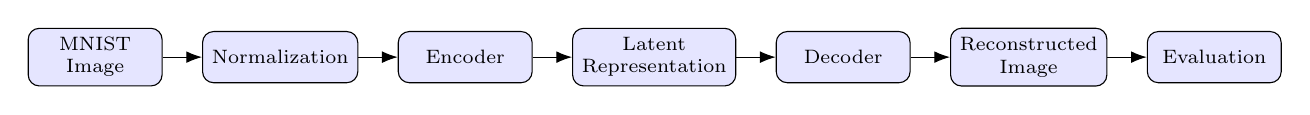
\begin{tikzpicture}[node distance=5mm]
\node[layer](a){MNIST\\Image};
\node[layer,right=of a](b){Normalization};
\node[layer,right=of b](c){Encoder};
\node[layer,right=of c](d){Latent\\Representation};
\node[layer,right=of d](e){Decoder};
\node[layer,right=of e](f){Reconstructed\\Image};
\node[layer,right=of f](g){Evaluation};

\foreach \x/\y in {a/b,b/c,c/d,d/e,e/f,f/g}
\draw[arrow](\x)--(\y);
\end{tikzpicture}
\end{center}

The experiment consists of four related studies:

\begin{enumerate}
\item Fully Connected Autoencoder
\item Convolutional Autoencoder
\item Denoising Convolutional Autoencoder
\item Variational Autoencoder
\end{enumerate}

%%%%%%%%%%%%%%%%%%%%%%%%%%%%%%%%%%%%%%%%%%%%%%%%%%%%%%%%%%%%
\section*{6. Exploring Autoencoders}

An autoencoder learns to reproduce its input at the output.

The encoder maps the input to a lower-dimensional representation:

\[
z=f_{\theta}(x),
\]

and the decoder reconstructs the input:

\[
\hat{x}=g_{\phi}(z).
\]

The training objective is to minimize reconstruction error:

\[
\mathcal{L}_{rec}
=
\frac{1}{N}\sum_{i=1}^{N}
\|x_i-\hat{x}_i\|^2.
\]

\begin{center}
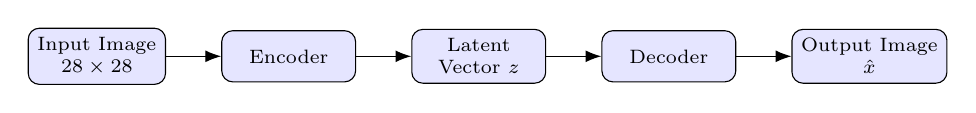
\begin{tikzpicture}[node distance=7mm]
\node[layer](a){Input Image\\$28\times28$};
\node[layer,right=of a](b){Encoder};
\node[layer,right=of b](c){Latent\\Vector $z$};
\node[layer,right=of c](d){Decoder};
\node[layer,right=of d](e){Output Image\\$\hat{x}$};

\foreach \x/\y in {a/b,b/c,c/d,d/e}
\draw[arrow](\x)--(\y);
\end{tikzpicture}
\end{center}

The latent vector is a compressed representation of the input.

%%%%%%%%%%%%%%%%%%%%%%%%%%%%%%%%%%%%%%%%%%%%%%%%%%%%%%%%%%%%
\section*{7. Fully Connected Autoencoder}

Flatten each image from

\[
28\times28=784
\]

to a vector of length 784.

Use the following architecture:

\begin{center}
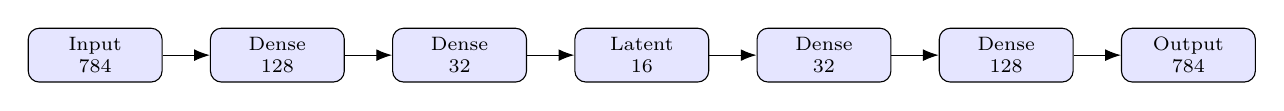
\begin{tikzpicture}[node distance=6mm]
\node[layer](a){Input\\784};
\node[layer,right=of a](b){Dense\\128};
\node[layer,right=of b](c){Dense\\32};
\node[layer,right=of c](d){Latent\\16};
\node[layer,right=of d](e){Dense\\32};
\node[layer,right=of e](f){Dense\\128};
\node[layer,right=of f](g){Output\\784};

\foreach \x/\y in {a/b,b/c,c/d,d/e,e/f,f/g}
\draw[arrow](\x)--(\y);
\end{tikzpicture}
\end{center}

Use ReLU activation in hidden layers and sigmoid activation in the output
layer.

\textbf{Suggested configuration:}

\begin{center}
\begin{tabular}{|l|l|}
\hline
Parameter & Value\\
\hline
Latent dimension & 16\\
Optimizer & Adam\\
Learning rate & $10^{-3}$\\
Batch size & 128\\
Epochs & 20\\
Loss & Binary Cross-Entropy\\
\hline
\end{tabular}
\end{center}

%%%%%%%%%%%%%%%%%%%%%%%%%%%%%%%%%%%%%%%%%%%%%%%%%%%%%%%%%%%%
\section*{8. Analysis of the Basic Autoencoder}

\textbf{Plot 1: Original versus Reconstructed Images}

\begin{figure}[H]
\centering
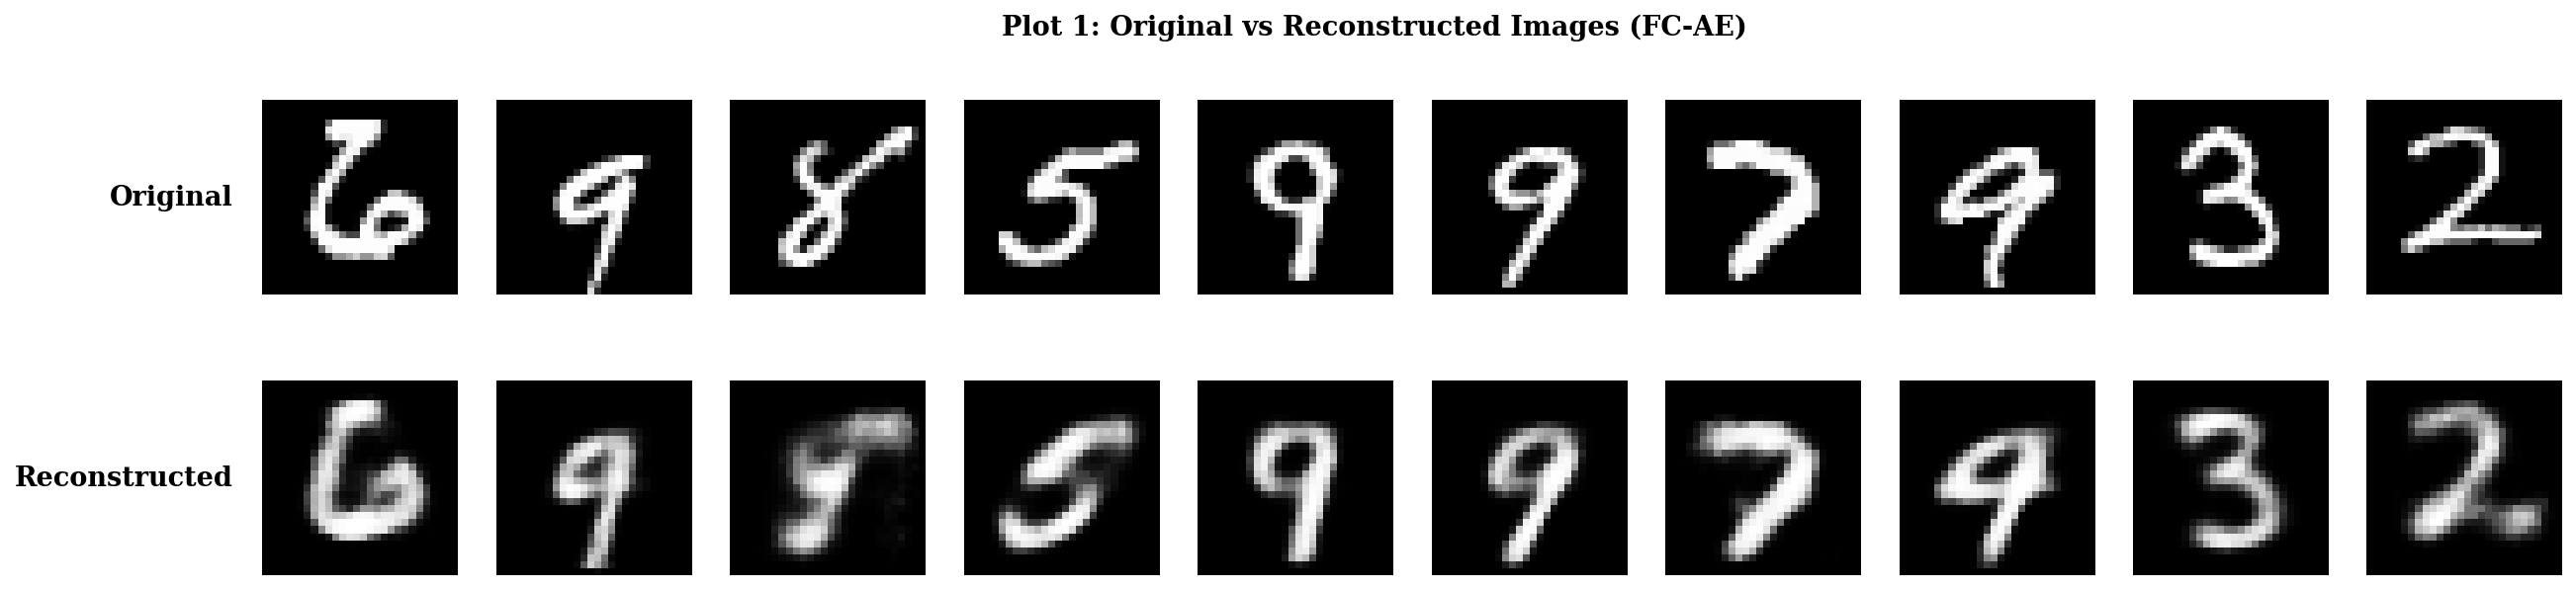
\includegraphics[width=0.95\textwidth]{figures/plot1_fc_original_vs_reconstructed.png}
\caption{Original versus reconstructed images for the fully connected autoencoder (test set).}
\end{figure}

The original shape of the digits is somewhat maintained and reconstructed. The reconstructed digit images are not as sharp as the original ones. Reconstruction suffers with curved parts of the images, and performs poorly in reconstruction of those curves, while digits like 1 and 7 with lesser curves are reconstructed more clearly. Flattening the image to a 784 dimensional vector destroys neighbourhood property, and loses spatial information, which causes it to suffer in the curved parts. The FC-AE gets the gist of a digit, not the fine strokes.\\\\

\textbf{Plot 2: Training and Validation Reconstruction Loss}

\begin{figure}[H]
\centering
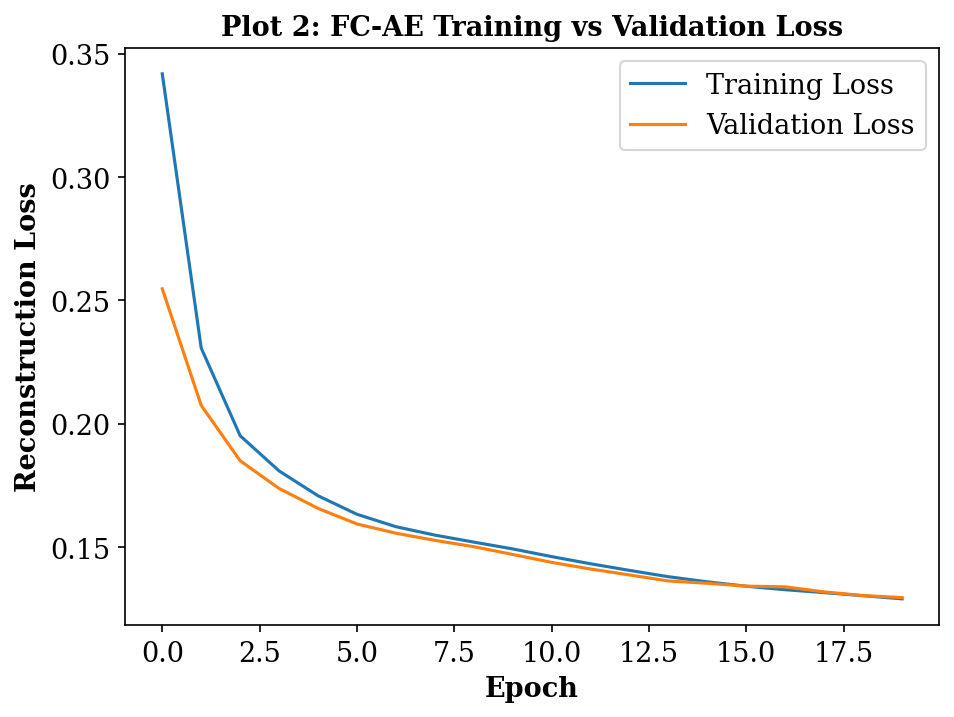
\includegraphics[width=0.6\textwidth]{figures/plot2_fc_training_validation_loss.png}
\caption{Training and validation reconstruction loss (binary cross-entropy) for the fully connected autoencoder over 20 epochs.}
\end{figure}

Both training and validation loss decrease sharply in the first few epochs, and then flatten at around epoch 20. Both curves almost overlap from around epoch 7.5. This shows that that model has converged well, and there is no overfitting, as there is no large gap between these two curves.

%%%%%%%%%%%%%%%%%%%%%%%%%%%%%%%%%%%%%%%%%%%%%%%%%%%%%%%%%%%%
\section*{9. Reconstruction Metrics}

Students must calculate the following metrics on the test set.

\subsection*{Mean Squared Error}

\[
MSE=
\frac{1}{N}
\sum_{i=1}^{N}
(x_i-\hat{x}_i)^2.
\]

\subsection*{Mean Absolute Error}

\[
MAE=
\frac{1}{N}
\sum_{i=1}^{N}
|x_i-\hat{x}_i|.
\]

\subsection*{Structural Similarity}

Calculate SSIM between the original and reconstructed images.

The implementation may use:

\url{https://scikit-image.org/docs/stable/api/skimage.metrics.html}

Report:

\begin{center}
\begin{tabular}{|l|c|}
\hline
Metric & Value\\
\hline
Test MSE & 0.022250\\
Test MAE & 0.059545\\
Mean SSIM & 0.748152\\
\hline
\end{tabular}
\end{center}

%%%%%%%%%%%%%%%%%%%%%%%%%%%%%%%%%%%%%%%%%%%%%%%%%%%%%%%%%%%%
\section*{10. Convolutional Autoencoder}

A Convolutional Autoencoder preserves spatial structure and uses convolutional
operations in the encoder and upsampling/transposed convolution operations
in the decoder.

The conceptual architecture is:

\begin{center}
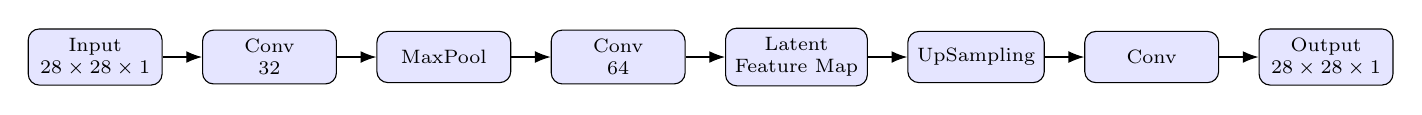
\begin{tikzpicture}[node distance=5mm]
\node[layer](a){Input\\$28\times28\times1$};
\node[layer,right=of a](b){Conv\\32};
\node[layer,right=of b](c){MaxPool};
\node[layer,right=of c](d){Conv\\64};
\node[layer,right=of d](e){Latent\\Feature Map};
\node[layer,right=of e](f){UpSampling};
\node[layer,right=of f](g){Conv};
\node[layer,right=of g](h){Output\\$28\times28\times1$};

\foreach \x/\y in {a/b,b/c,c/d,d/e,e/f,f/g,g/h}
\draw[arrow](\x)--(\y);
\end{tikzpicture}
\end{center}

A possible implementation is:

\begin{verbatim}
Input(28,28,1)
Conv2D(32, 3, activation='relu', padding='same')
MaxPooling2D(2, padding='same')
Conv2D(64, 3, activation='relu', padding='same')
MaxPooling2D(2, padding='same')
Conv2D(64, 3, activation='relu', padding='same')
UpSampling2D(2)
Conv2D(32, 3, activation='relu', padding='same')
UpSampling2D(2)
Conv2D(1, 3, activation='sigmoid', padding='same')
\end{verbatim}

The exact implementation may use Conv2DTranspose instead of UpSampling2D.

%%%%%%%%%%%%%%%%%%%%%%%%%%%%%%%%%%%%%%%%%%%%%%%%%%%%%%%%%%%%
\section*{11. Comparing Fully Connected and Convolutional Autoencoders}

Train both models using the same training and test images.

\begin{center}
\begin{tabular}{|l|c|c|c|c|}
\hline
Model & MSE & MAE & SSIM & Parameters\\
\hline
Fully Connected AE & 0.022250 & 0.059545 & 0.748152 & 211{,}040\\
Convolutional AE & 0.002479 & 0.015027 & 0.974972 & 74{,}497\\
\hline
\end{tabular}
\end{center}

\vspace{20mm}

\textbf{Plot 3: Reconstruction Comparison}

\begin{figure}[H]
\centering
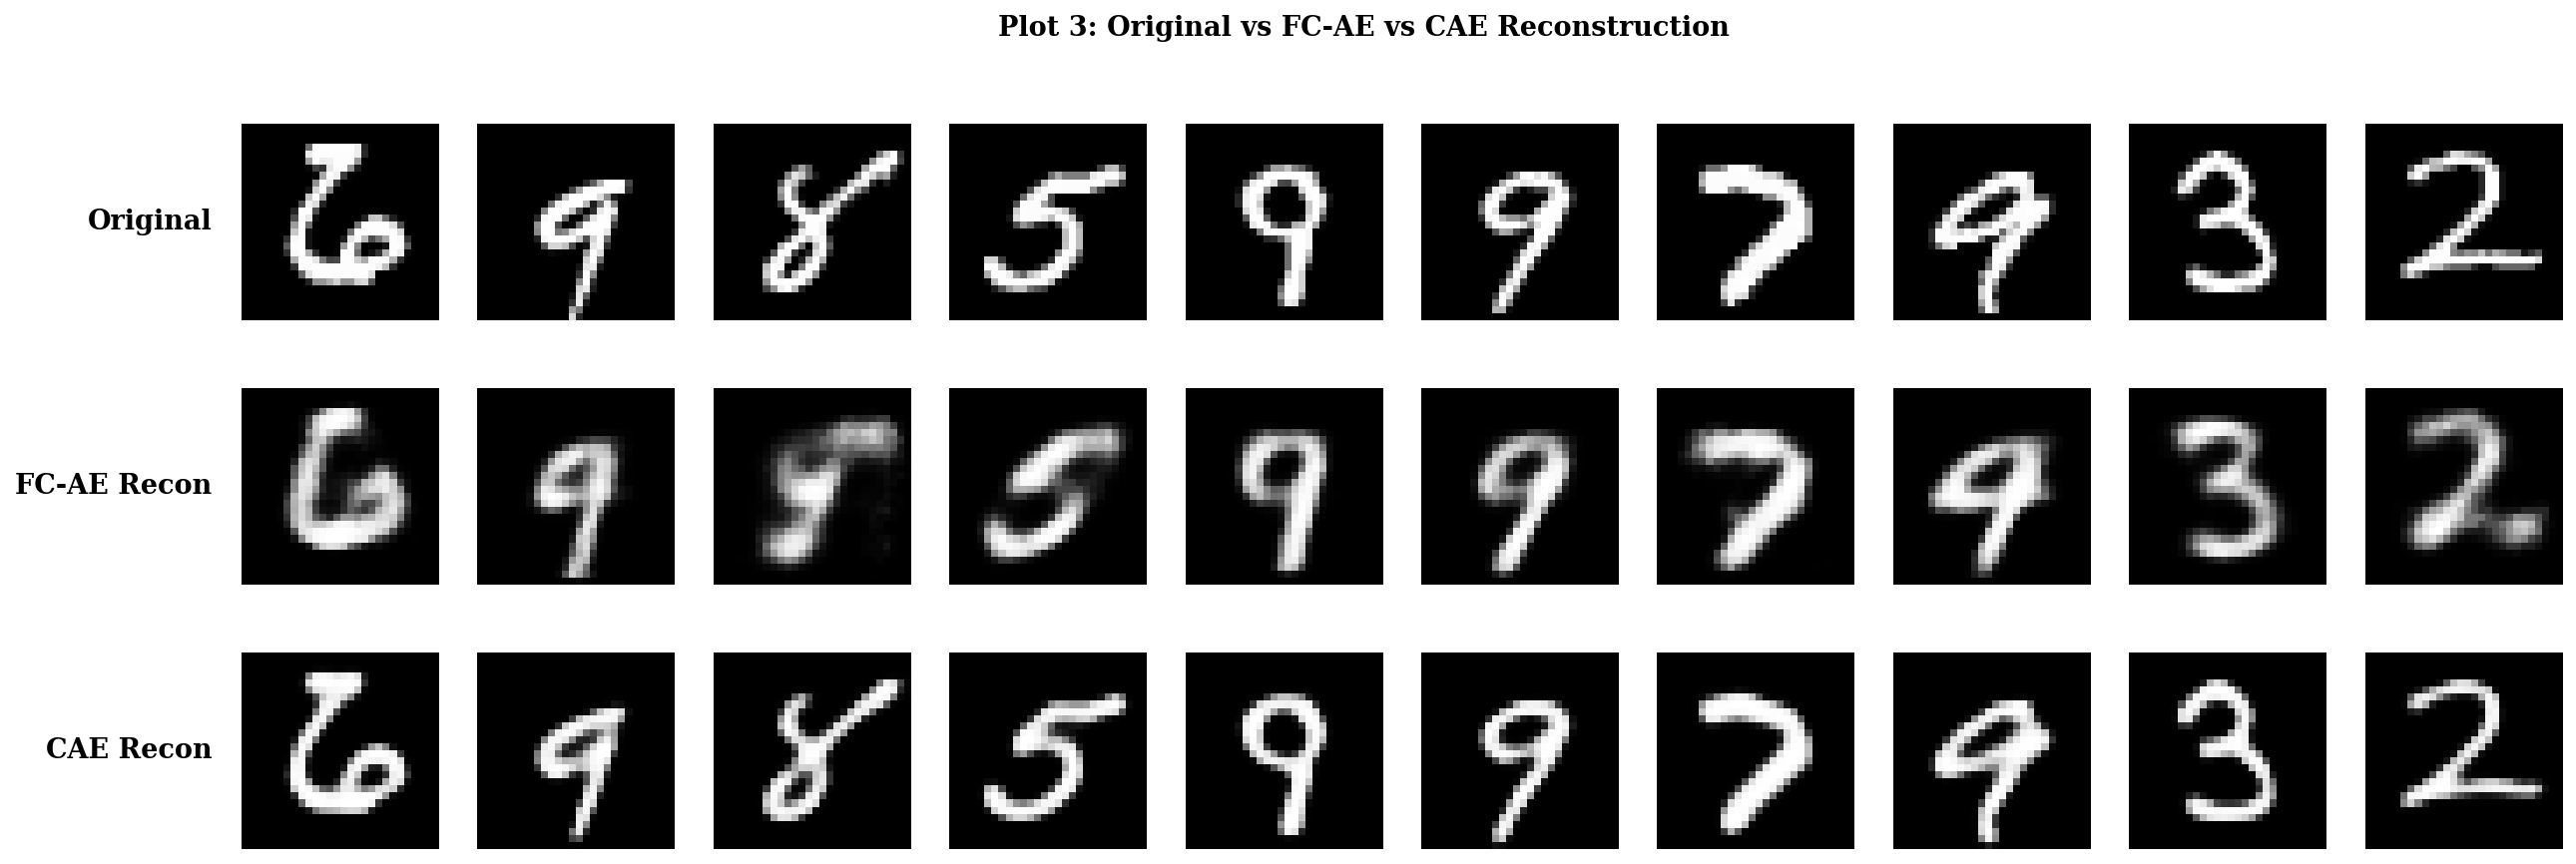
\includegraphics[width=0.95\textwidth]{figures/plot3_fc_vs_cae_reconstruction.png}
\caption{Original image versus FC-AE reconstruction versus CAE reconstruction.}
\end{figure}

CAE reconstructions are sharper than FC-AE reconstructions, and is a closer match to the original input image. This is also supported by the MSE values of both, where FC-AE gets 0.02225, while CAE gets 0.00248, which is nearly 10x smaller error. Convolution and pooling maintain neighbourhood property and preserve spatial information, hence it performs better than FC-AE on curves as we saw FC-AE loses spatial information. 

%%%%%%%%%%%%%%%%%%%%%%%%%%%%%%%%%%%%%%%%%%%%%%%%%%%%%%%%%%%%
\section*{12. Denoising Autoencoder}

A denoising autoencoder receives a corrupted image but is trained to
reconstruct the original clean image.

The training mapping is:

\[
\boxed{\tilde{x}\rightarrow\text{Encoder}\rightarrow z
\rightarrow\text{Decoder}\rightarrow\hat{x}}
\]

where $\tilde{x}$ is a noisy version of the clean image $x$.

\begin{center}
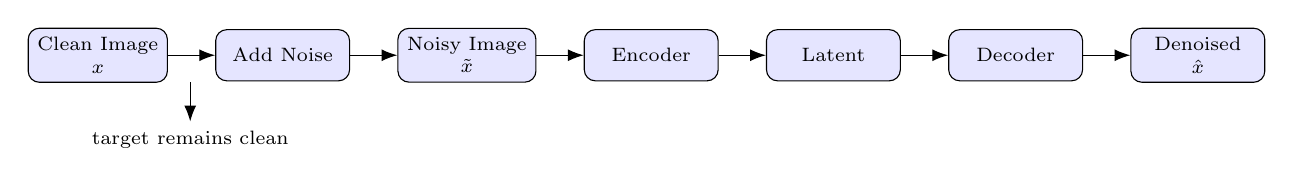
\begin{tikzpicture}[node distance=6mm]
\node[layer](a){Clean Image\\$x$};
\node[layer,right=of a](b){Add Noise};
\node[layer,right=of b](c){Noisy Image\\$\tilde{x}$};
\node[layer,right=of c](d){Encoder};
\node[layer,right=of d](e){Latent};
\node[layer,right=of e](f){Decoder};
\node[layer,right=of f](g){Denoised\\$\hat{x}$};

\foreach \x/\y in {a/b,b/c,c/d,d/e,e/f,f/g}
\draw[arrow](\x)--(\y);

\draw[arrow]($(a.south)!0.5!(b.south)$) -- ++(0,-5mm)
node[below,font=\scriptsize]{target remains clean};
\end{tikzpicture}
\end{center}

%%%%%%%%%%%%%%%%%%%%%%%%%%%%%%%%%%%%%%%%%%%%%%%%%%%%%%%%%%%%
\section*{13. Adding Image Noise}

Use at least two corruption types.

\subsection*{Gaussian Noise}

\[
\tilde{x}=x+n,
\qquad
n\sim\mathcal{N}(0,\sigma^2).
\]

Suggested standard deviations:

\[
\sigma\in\{0.1,0.2,0.3\}.
\]

Clip the resulting image to the range $[0,1]$.

\subsection*{Salt-and-Pepper Noise}

Randomly replace a small proportion of pixels with values close to 0 or 1.

Suggested corruption levels:

\[
p\in\{0.05,0.10,0.20\}.
\]

%%%%%%%%%%%%%%%%%%%%%%%%%%%%%%%%%%%%%%%%%%%%%%%%%%%%%%%%%%%%
\section*{14. Denoising Plots}

\textbf{Plot 4: Clean vs. Noisy vs. Denoised}

\begin{figure}[H]
\centering
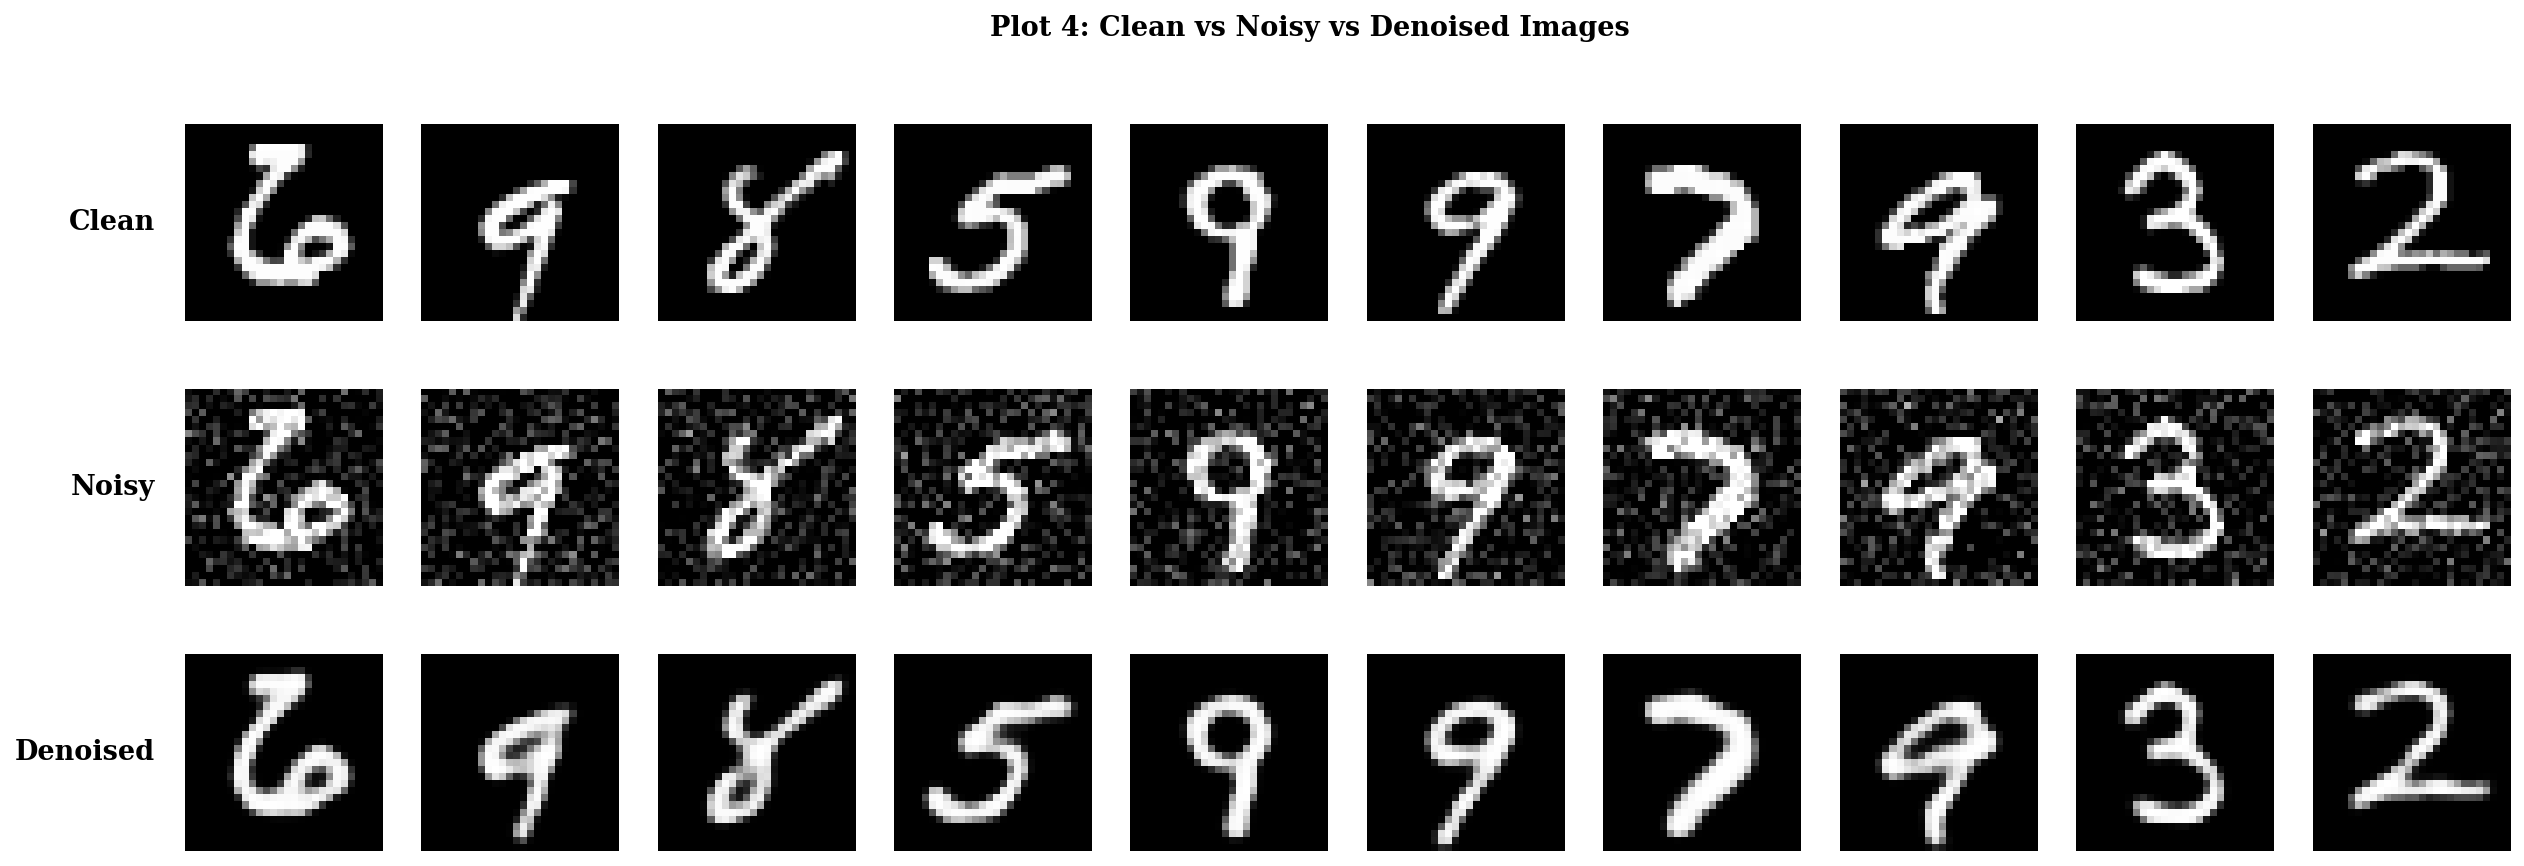
\includegraphics[width=0.95\textwidth]{figures/plot4_clean_noisy_denoised.png}
\caption{Clean, noisy (Gaussian, $\sigma=0.2$), and denoised images for the denoising convolutional autoencoder.}
\end{figure}

Noisy images have multiple grain like dots on them, i.e the noise. The digits are readable, but the noisy pattern makes it slightly uncomfortable. Denoised image removes the noise from these noisy images, and almost produces the input clean image back, removing almost all noise. This shows that denoising autoencoders learn to remove the noise out, instead of learning them like patterns.\\\\

\textbf{Plot 5: Noise Level vs. Reconstruction Quality}

\begin{figure}[H]
\centering
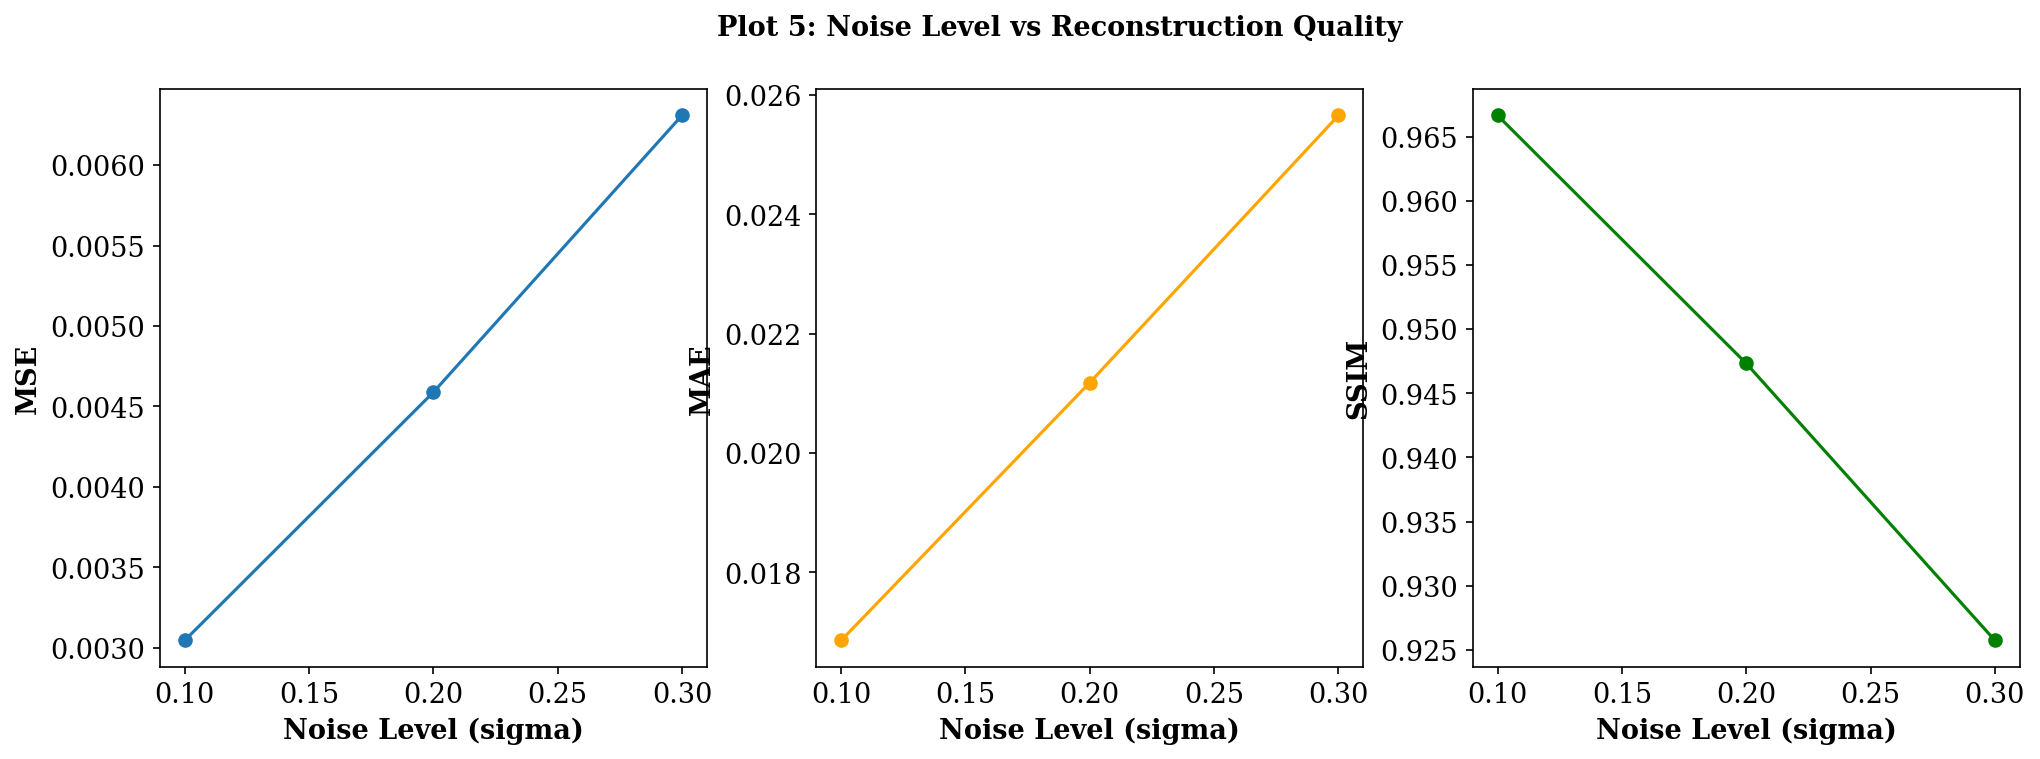
\includegraphics[width=0.95\textwidth]{figures/plot5_noise_level_vs_quality.png}
\caption{MSE, MAE and SSIM of the denoising CAE as a function of Gaussian noise level $\sigma$.}
\end{figure}

Report:

\begin{center}
\begin{tabular}{|c|c|c|c|}
\hline
Noise Level & MSE & MAE & SSIM\\
\hline
0.1 & 0.003045 & 0.016856 & 0.966647\\
0.2 & 0.004588 & 0.021180 & 0.947325\\
0.3 & 0.006309 & 0.025659 & 0.925741\\
\hline
\end{tabular}
\end{center}

MSE and MAE increase steadily with increase in $\sigma$ from 0.1 to 0.3, and SSIM decrease steadily in the same interval of $\sigma$ . With more noise, true pixel values get wiped out, hence the model suffers to reconstruct the original image, which is why the errors increase with noise. But, since SSIM is always above 0.92, the model still keeps the digit's structure properly, even with the highest noise.

%%%%%%%%%%%%%%%%%%%%%%%%%%%%%%%%%%%%%%%%%%%%%%%%%%%%%%%%%%%%

\vspace{10mm}

\section*{15. Variational Autoencoder}

A conventional autoencoder maps an input to a deterministic latent vector:

\[
z=f(x).
\]

A VAE instead learns a probability distribution:

\[
q_{\phi}(z|x)
=
\mathcal{N}
\left(
\mu(x),
\operatorname{diag}(\sigma^2(x))
\right).
\]

The encoder produces:

\[
\mu,\qquad \log\sigma^2.
\]

A latent vector is sampled using the reparameterization trick:

\[
z=\mu+\sigma\odot\epsilon,
\qquad
\epsilon\sim\mathcal{N}(0,I).
\]

\begin{center}
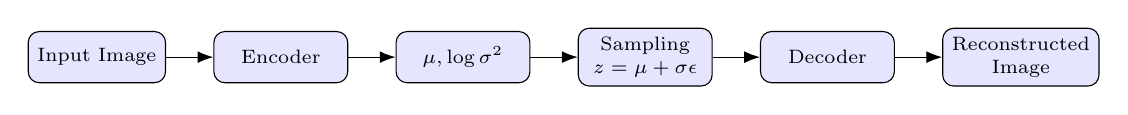
\begin{tikzpicture}[node distance=6mm]
\node[layer](a){Input Image};
\node[layer,right=of a](b){Encoder};
\node[layer,right=of b](c){$\mu,\log\sigma^2$};
\node[layer,right=of c](d){Sampling\\$z=\mu+\sigma\epsilon$};
\node[layer,right=of d](e){Decoder};
\node[layer,right=of e](f){Reconstructed\\Image};

\foreach \x/\y in {a/b,b/c,c/d,d/e,e/f}
\draw[arrow](\x)--(\y);
\end{tikzpicture}
\end{center}

%%%%%%%%%%%%%%%%%%%%%%%%%%%%%%%%%%%%%%%%%%%%%%%%%%%%%%%%%%%%
\section*{16. VAE Loss Function}

The VAE objective consists of two components.

\subsection*{Reconstruction Loss}

\[
\mathcal{L}_{rec}
=
-\mathbb{E}_{q_{\phi}(z|x)}
[\log p_{\theta}(x|z)].
\]

For normalized MNIST images, binary cross-entropy can be used.

\subsection*{KL Divergence}

\[
D_{KL}
\left(
q_{\phi}(z|x)\parallel p(z)
\right)
=
-\frac{1}{2}
\sum_j
\left(
1+\log\sigma_j^2-\mu_j^2-\sigma_j^2
\right).
\]

The total loss is

\[
\boxed{
\mathcal{L}_{VAE}
=
\mathcal{L}_{rec}
+
\mathcal{L}_{KL}
}
\]

where the prior is usually

\[
p(z)=\mathcal{N}(0,I).
\]

%%%%%%%%%%%%%%%%%%%%%%%%%%%%%%%%%%%%%%%%%%%%%%%%%%%%%%%%%%%%
\section*{17. VAE Implementation}

Use a small latent space so that it can be visualized.

Suggested latent dimension:

\[
z\in\mathbb{R}^{2}.
\]

The encoder should produce:

\[
\mu\in\mathbb{R}^{2},
\qquad
\log\sigma^2\in\mathbb{R}^{2}.
\]

The decoder maps

\[
z\rightarrow28\times28\times1.
\]

A compact architecture is:

\begin{center}
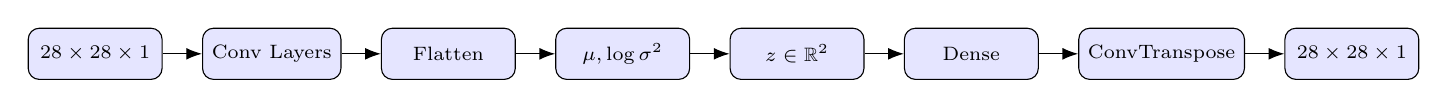
\begin{tikzpicture}[node distance=5mm]
\node[layer](a){$28\times28\times1$};
\node[layer,right=of a](b){Conv Layers};
\node[layer,right=of b](c){Flatten};
\node[layer,right=of c](d){$\mu,\log\sigma^2$};
\node[layer,right=of d](e){$z\in\mathbb{R}^2$};
\node[layer,right=of e](f){Dense};
\node[layer,right=of f](g){ConvTranspose};
\node[layer,right=of g](h){$28\times28\times1$};

\foreach \x/\y in {a/b,b/c,c/d,d/e,e/f,f/g,g/h}
\draw[arrow](\x)--(\y);
\end{tikzpicture}
\end{center}

%%%%%%%%%%%%%%%%%%%%%%%%%%%%%%%%%%%%%%%%%%%%%%%%%%%%%%%%%%%%
\section*{18. Exploring the VAE Latent Space}

Since the latent dimension is two, students can visualize the encoded test images in a two-dimensional plane.\\

\textbf{Plot 6: VAE Latent Space}

\begin{figure}[H]
\centering
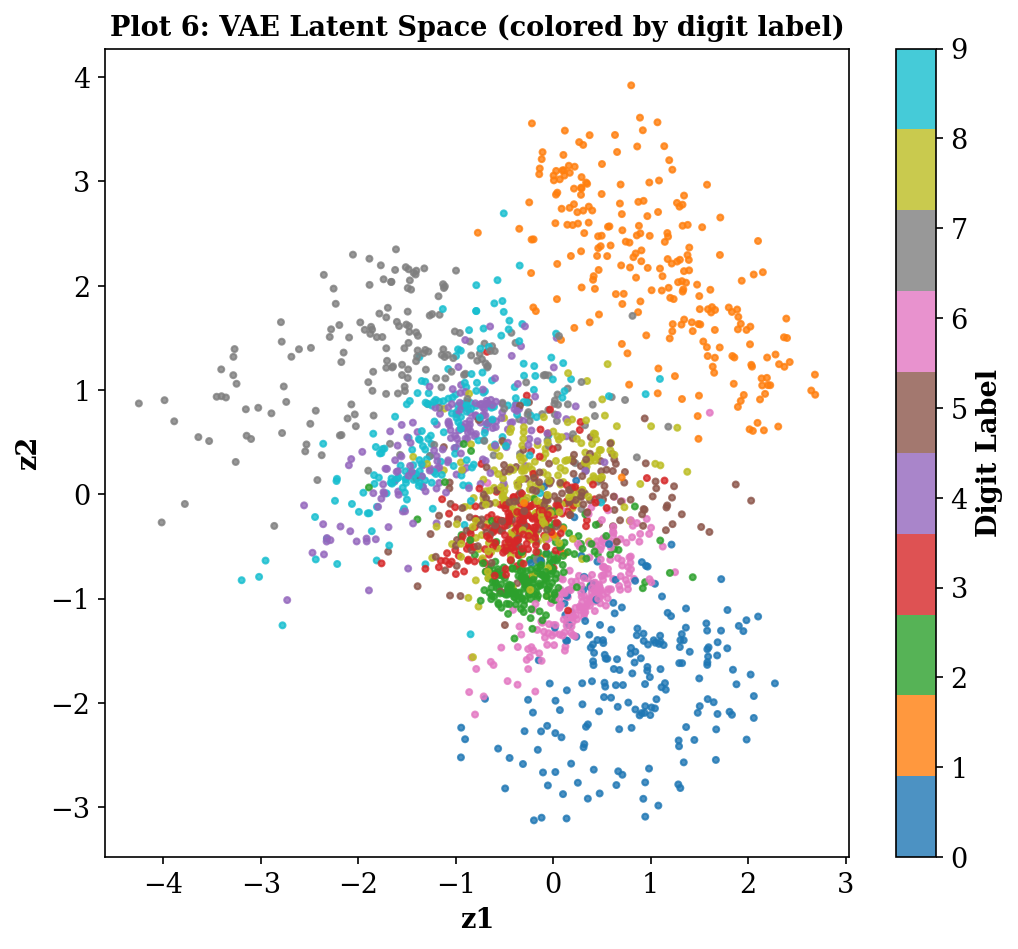
\includegraphics[width=0.65\textwidth]{figures/plot6_vae_latent_space.png}
\caption{2D VAE latent space of the test set, colored by digit label.}
\end{figure}

Digits belonging to same class are mostly in the same part of the plane and form loose clusters, even though the model never saw the labels during training. The encoder groups inputs by how similar they look, so digits with similar strokes have similar $\mu$ values. Clusters which look similar, (like 3 and 8, or 1 and 7, etc) overlap near the edges of their clusters, and digits with lesser similarities are clearly separated.

%%%%%%%%%%%%%%%%%%%%%%%%%%%%%%%%%%%%%%%%%%%%%%%%%%%%%%%%%%%%
\section*{19. Generating New Images with the VAE}

Sample points from

\[
z\sim\mathcal{N}(0,I).
\]

Pass the sampled latent vectors through the decoder.\\

\textbf{Plot 7: Randomly Generated Images}

\begin{figure}[H]
\centering
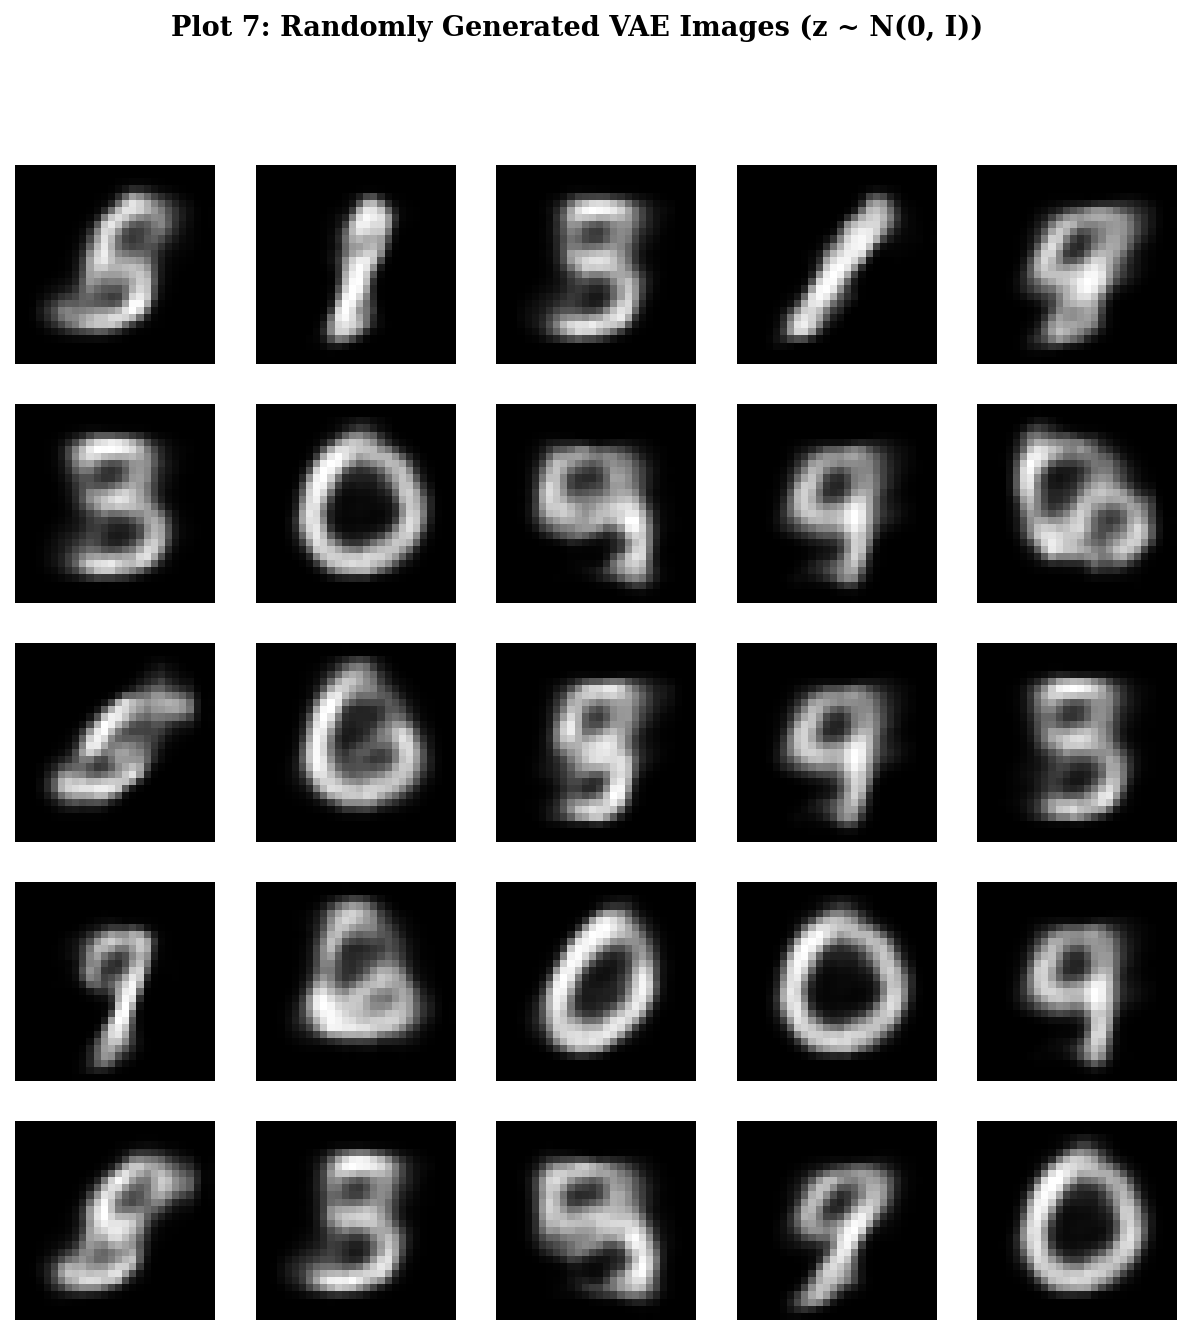
\includegraphics[width=0.55\textwidth]{figures/plot7_vae_generated_images.png}
\caption{25 images generated by decoding latent vectors sampled from $\mathcal{N}(0,I)$.}
\end{figure}

Most of the generated digits look similar to real images, with legible handwriting and somewhat recognizable. Few samples came out really blurred, and unrecognizeable, like images 10th, 12th and 17th images. This blur happens because the model confuses similar looking digits, espceially the ones which overlapped clusters in the previous plot.

%%%%%%%%%%%%%%%%%%%%%%%%%%%%%%%%%%%%%%%%%%%%%%%%%%%%%%%%%%%%
\section*{20. Latent Space Interpolation}

Select two latent vectors:

\[
z_A,\qquad z_B.
\]

Construct

\[
z(\alpha)=(1-\alpha)z_A+\alpha z_B,
\qquad
\alpha\in[0,1].
\]

Use values such as:

\[
\alpha=
0,\;0.1,\;0.2,\ldots,1.
\]

Decode every interpolated vector.\\

\textbf{Plot 8: Latent Space Interpolation}

\begin{figure}[H]
\centering
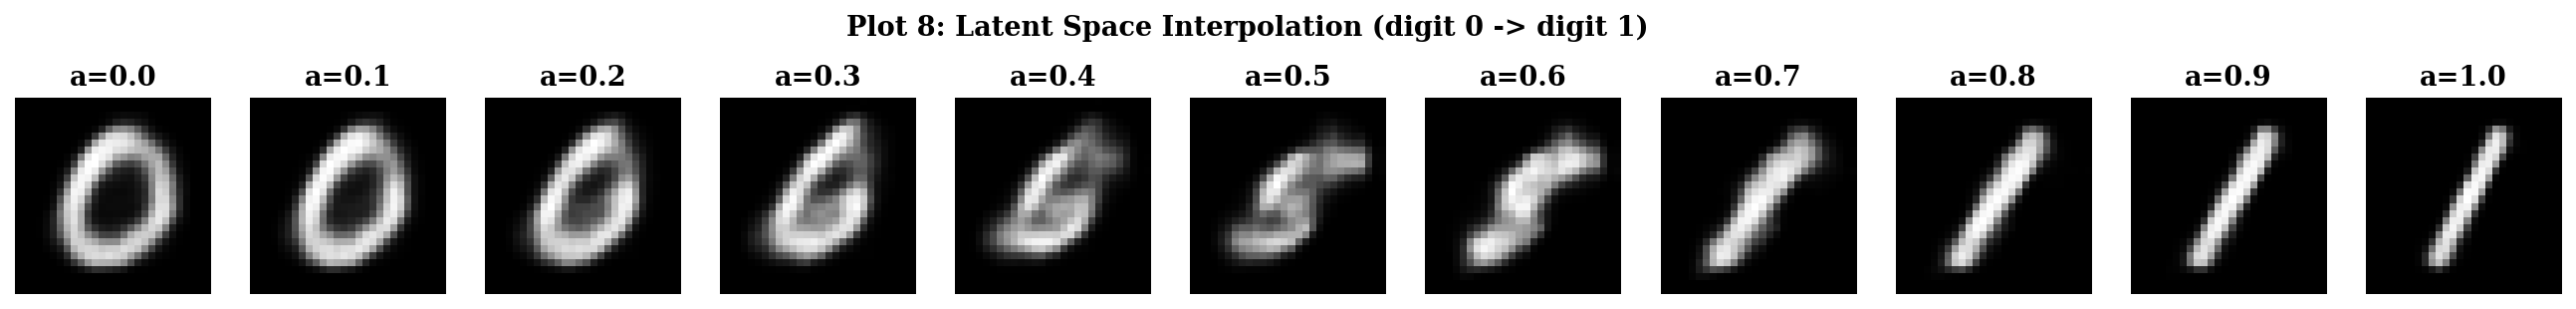
\includegraphics[width=0.95\textwidth]{figures/plot8_vae_latent_interpolation.png}
\caption{Latent-space interpolation from the encoded latent mean of a digit 0 to that of a digit 1, $\alpha=0$ to $1$ in steps of 0.1.}
\end{figure}

As $\alpha$ moves from 0 to 1, the digit 0 transforms into the digit 1 gradually. There is no sudden change in shape. Nearby points in latent space decode to form similar images, and the latent space is continuous for VAEs.

%%%%%%%%%%%%%%%%%%%%%%%%%%%%%%%%%%%%%%%%%%%%%%%%%%%%%%%%%%%%
\section*{21. Reconstruction Comparison Across Models}

Compare the three reconstruction-based models:

\begin{center}
\begin{tabular}{|l|c|c|c|c|}
\hline
Model & MSE & MAE & SSIM & Parameters\\
\hline
Fully Connected AE & 0.022250 & 0.059545 & 0.748152 & 211{,}040\\
Convolutional AE & 0.002479 & 0.015027 & 0.974972 & 74{,}497\\
Denoising CAE & 0.004558 & 0.021023 & 0.947821 & 74{,}497\\
\hline
\end{tabular}
\end{center}

For the VAE, report its reconstruction loss separately because its total
objective also contains the KL-divergence term.

\begin{center}
\begin{tabular}{|l|c|}
\hline
VAE Metric & Value\\
\hline
Reconstruction Loss & 151.665497\\
KL Loss & 5.489002\\
Total Loss & 157.154495\\
Test MSE & 0.044263\\
Test MAE & 0.102603\\
Mean SSIM & 0.507384\\
\hline
\end{tabular}
\end{center}

%%%%%%%%%%%%%%%%%%%%%%%%%%%%%%%%%%%%%%%%%%%%%%%%%%%%%%%%%%%%
\section*{22. Reconstruction Error Distribution}

Calculate the per-image reconstruction error:

\[
e_i=
\frac{1}{D}
\sum_{j=1}^{D}
(x_{ij}-\hat{x}_{ij})^2.
\]

\textbf{Plot 9: Distribution of Reconstruction Errors}

\begin{figure}[H]
\centering
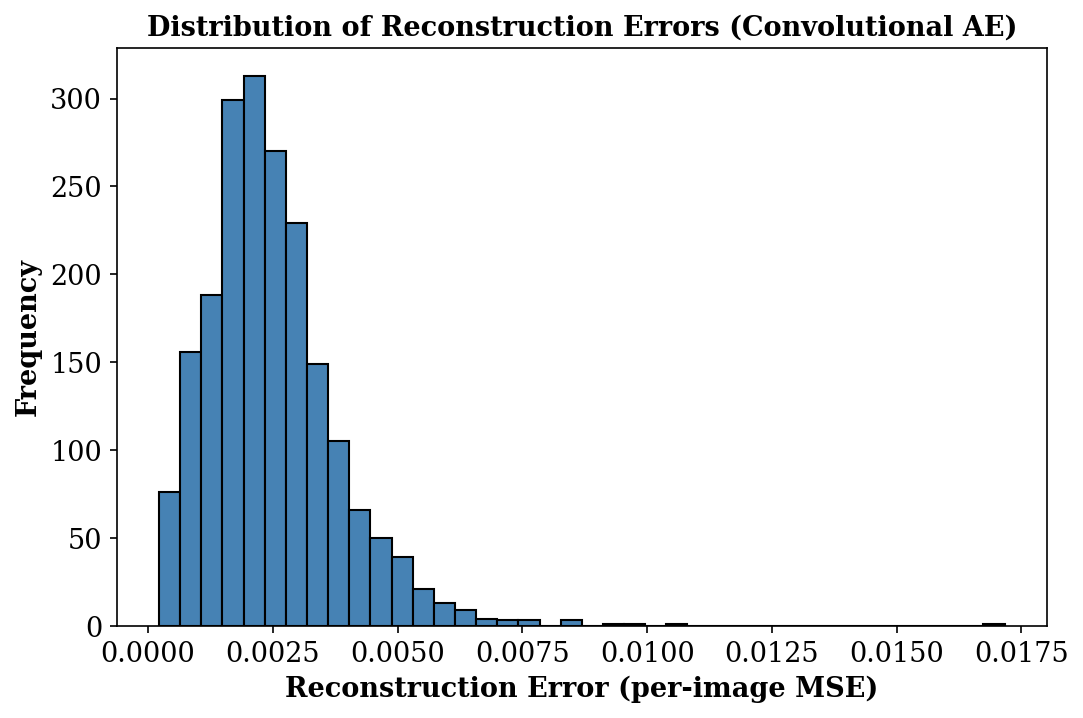
\includegraphics[width=0.65\textwidth]{figures/plot_error_distribution.png}
\caption{Histogram of per-image reconstruction error (MSE) on the test set, Convolutional AE.}
\end{figure}

The bars in the histogram are dense and high at around the mean MSE of the model (0.00248), and later decreases with increase in error. This shows that most images are reconstructed clearly, and few hard images cause errors, like 6 and 8, which have similar features and are harder for the model to distinguish.

%%%%%%%%%%%%%%%%%%%%%%%%%%%%%%%%%%%%%%%%%%%%%%%%%%%%%%%%%%%%
\section*{23. High-Error Image Analysis}

Select the five test images having the largest reconstruction errors.

\begin{figure}[H]
\centering
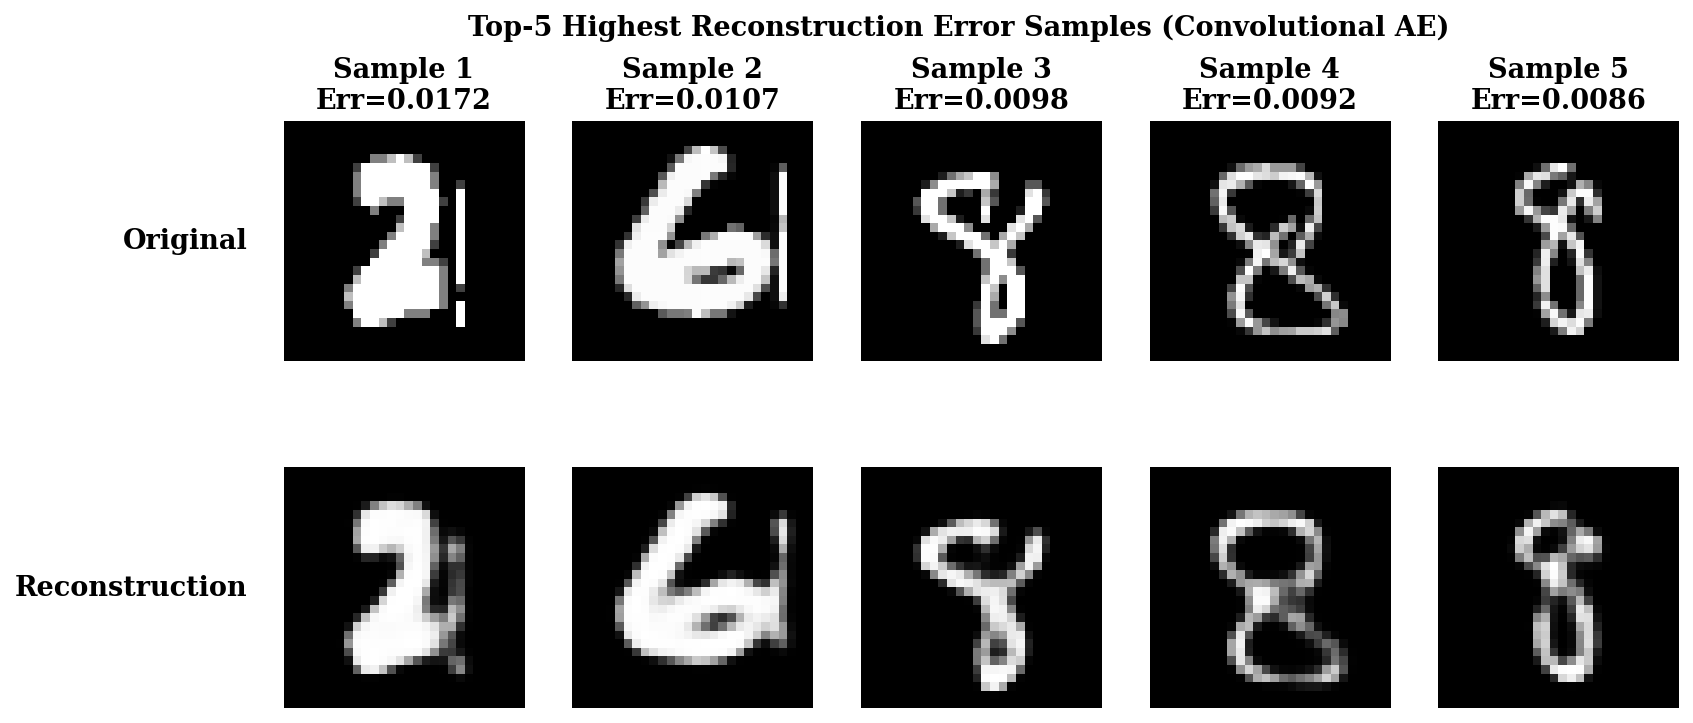
\includegraphics[width=0.8\textwidth]{figures/plot_high_error_samples.png}
\caption{Top-5 highest reconstruction-error test images (Convolutional AE) with their reconstructions.}
\end{figure}

\begin{center}
\begin{tabular}{|c|c|c|c|}
\hline
Sample & Test Index & True Label & Reconstruction Error (MSE)\\
\hline
1 & 1670 & 2 & 0.017161\\
2 & 97 & 6 & 0.010745\\
3 & 417 & 8 & 0.009759\\
4 & 262 & 8 & 0.009177\\
5 & 1327 & 8 & 0.008607\\
\hline
\end{tabular}
\end{center}

Four of the five hardest samples are 8s; their overlapping loops carry more detail than the compressed latent code can hold. The fifth is an unusually written 2 that departs from the typical stroke pattern. Both point to the same cause: digits with complex or atypical shapes carry more information than the bottleneck can preserve, so they land with higher error than plainer digit styles.

%%%%%%%%%%%%%%%%%%%%%%%%%%%%%%%%%%%%%%%%%%%%%%%%%%%%%%%%%%%%
\section*{24. Consolidated Results}

\begin{center}
\begin{tabular}{|l|c|c|c|c|c|}
\hline
Model & MSE & MAE & SSIM & Parameters & Time (s)\\
\hline
FC Autoencoder & 0.022250 & 0.059545 & 0.748152 & 211{,}040 & 11.65\\
Conv. Autoencoder & 0.002479 & 0.015027 & 0.974972 & 74{,}497 & 19.19\\
Denoising CAE & 0.004558 & 0.021023 & 0.947821 & 74{,}497 & 19.34\\
VAE & 0.044263 & 0.102603 & 0.507384 & 284{,}933 & 206.55\\
\hline
\end{tabular}
\end{center}

The values were obtained from the student's own execution (see Section 25 for source code).

%%%%%%%%%%%%%%%%%%%%%%%%%%%%%%%%%%%%%%%%%%%%%%%%%%%%%%%%%%%%
\section*{25. Source Code}

The repository contains a single Kaggle notebook implementing the complete pipeline described in this report, from data loading and preprocessing through the fully connected autoencoder, convolutional autoencoder, denoising autoencoder and variational autoencoder, including all required plots, metrics, and additional exercises:\\

    \hspace{25mm}  \url{https://github.com/Ashwin271206/dl-lab/tree/main/Lab%207}\\

The repository contains a single Kaggle notebook covering all tasks experimented in this report, along with the generated figures and outputs.

%%%%%%%%%%%%%%%%%%%%%%%%%%%%%%%%%%%%%%%%%%%%%%%%%%%%%%%%%%%%
\section*{26. Additional Latent-Dimension Study}

Repeat the basic autoencoder using:

\[
d_z\in\{2,8,16,32\}.
\]

Report:

\begin{center}
\begin{tabular}{|c|c|c|c|}
\hline
Latent Dimension & MSE & SSIM & Parameters\\
\hline
2 & 0.048572 & 0.459916 & 210{,}130\\
8 & 0.026562 & 0.703327 & 210{,}520\\
16 & 0.024345 & 0.728851 & 211{,}040\\
32 & 0.019325 & 0.780466 & 212{,}080\\
\hline
\end{tabular}
\end{center}

\textbf{Plot 10: Latent Dimension vs. Reconstruction MSE}

\begin{figure}[H]
\centering
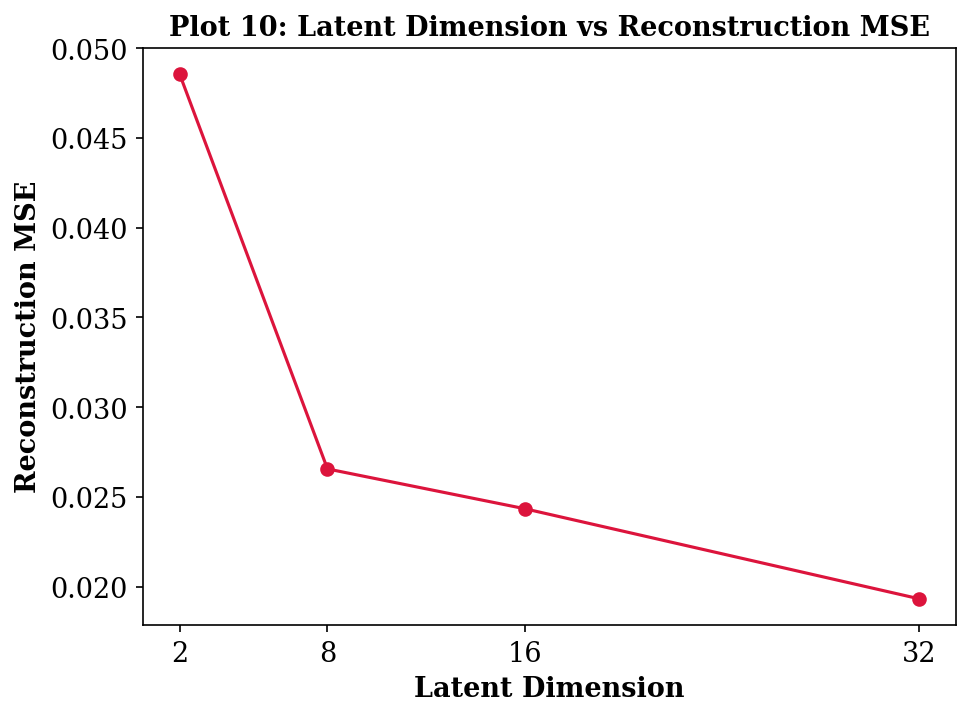
\includegraphics[width=0.6\textwidth]{figures/plot10_latent_dimension_vs_mse.png}
\caption{Fully connected AE: reconstruction MSE versus latent dimension.}
\end{figure}

MSE decreases steadily with increase in latent dimension from 2 to 32, while SSIM increases. Bigger latent space gives more opportunity for the encoder to preserve details instead of dropping them. Small bottlenecks require to compress heavily, hence losing information and causing blurred outputs, while slightly bigger bottlenecks help in preserving more information.

%%%%%%%%%%%%%%%%%%%%%%%%%%%%%%%%%%%%%%%%%%%%%%%%%%%%%%%%%%%%
\section*{27. Additional Exercises}

\subsection*{27.1 Convolutional AE with Latent Channels 4, 8, 16, 32}

Train the convolutional autoencoder with bottleneck channel widths of 4, 8, 16 and 32 and compare reconstruction quality.

\begin{center}
\begin{tabular}{|c|c|c|c|}
\hline
Latent Channels & MSE & MAE & SSIM\\
\hline
4 & 0.008560 & 0.029990 & 0.918833\\
8 & 0.005544 & 0.023280 & 0.944809\\
16 & 0.004067 & 0.019709 & 0.959489\\
32 & 0.003157 & 0.017041 & 0.966528\\
\hline
\end{tabular}
\end{center}

\begin{figure}[H]
\centering
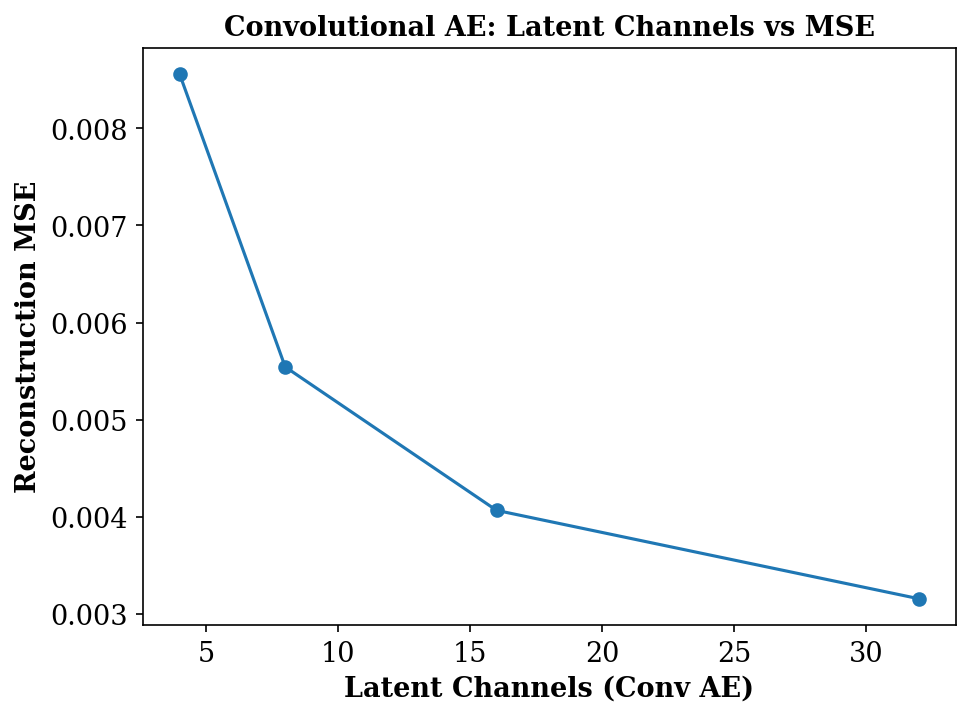
\includegraphics[width=0.6\textwidth]{figures/extra_conv_latent_channels_vs_mse.png}
\caption{Convolutional AE: reconstruction MSE versus number of bottleneck latent channels.}
\end{figure}

MSE decreases and SSIM increases with increase in latent channels, and the same tradeoff between compression and quality in the previous plot is shown. The narrowest CAE with 4 channels gets an SSIM of 0.919, which is still better than the 16 channel FC-AE which gets only 0.729 SSIM.

\subsection*{27.2 Gaussian Noise vs Salt-and-Pepper Noise}

Compare Gaussian noise ($\sigma=0.2$) and salt-and-pepper noise ($p=0.10$) using the same denoising architecture.

\begin{center}
\begin{tabular}{|l|c|c|c|}
\hline
Noise Type & MSE & MAE & SSIM\\
\hline
Gaussian ($\sigma=0.2$) & 0.004558 & 0.021023 & 0.947821\\
Salt-and-Pepper ($p=0.10$) & 0.005266 & 0.022243 & 0.942448\\
\hline
\end{tabular}
\end{center}

\begin{figure}[H]
\centering
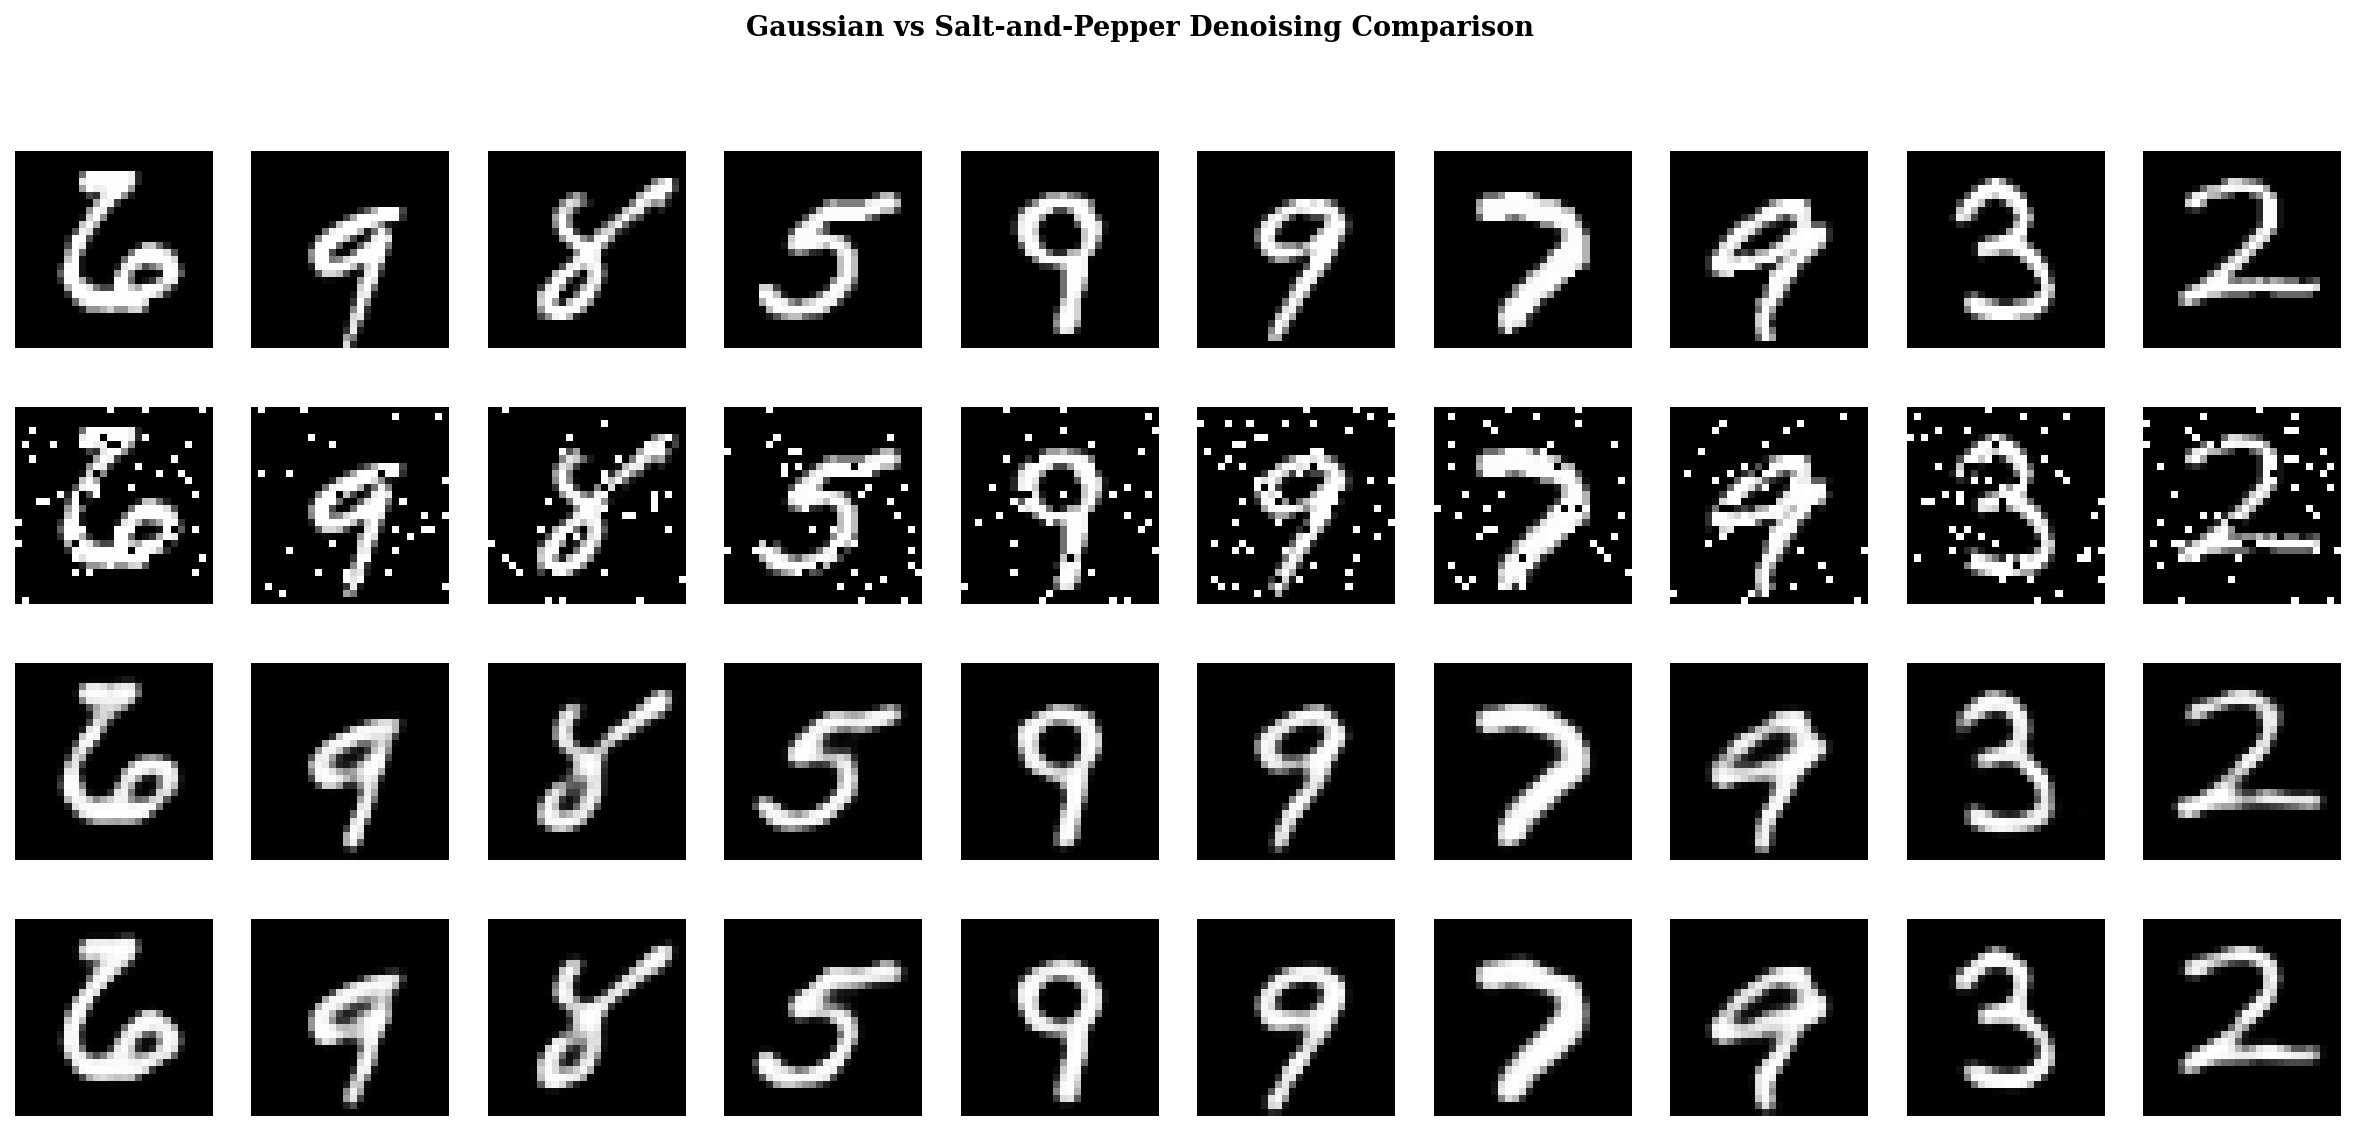
\includegraphics[width=0.95\textwidth]{figures/extra_gaussian_vs_saltpepper.png}
\caption{Clean, noisy, and denoised images under Gaussian noise versus salt-and-pepper noise.}
\end{figure}

SSIM is slightly higher for Gaussian noise, with 0,948, than for salt and pepper noise with 0.942. This can be caused, as salt and pepper heavily wipes out pixel data (0.948) than for salt-and-pepper (0.942) at these settings. Salt-and-pepper wipes a pixel out entirely; Gaussian noise only nudges it, leaving more residual signal for the network to use. Both noise types are handled well, with salt-and-pepper the marginally tougher case.

\subsection*{27.3 Denoising AE at Two Noise Levels}

Train the denoising autoencoder using two different noise levels and compare SSIM.

\begin{center}
\begin{tabular}{|c|c|c|c|}
\hline
Noise Level ($\sigma$) & MSE & MAE & SSIM\\
\hline
0.1 & 0.003051 & 0.016983 & 0.965097\\
0.3 & 0.006585 & 0.025967 & 0.921000\\
\hline
\end{tabular}
\end{center}

\begin{figure}[H]
\centering
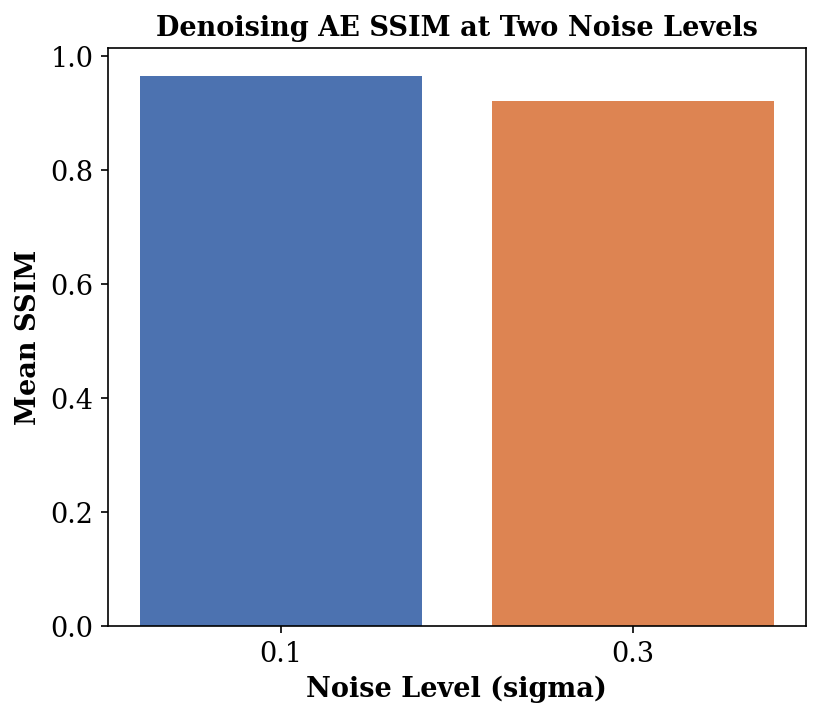
\includegraphics[width=0.5\textwidth]{figures/extra_denoising_ssim_two_levels.png}
\caption{Mean SSIM of the denoising CAE trained and evaluated at $\sigma=0.1$ versus $\sigma=0.3$.}
\end{figure}

SSIM is higher (0.965) for lower noise, and slightly drops to 0.921 with noise level 0.3. This is because more noise would override real pixels, and hence performs poorer, while lower noise makes the true pixels clearer..

\subsection*{27.4 Transposed Convolution Decoder vs UpSampling Decoder}

Replace the convolutional decoder's UpSampling2D layers with Conv2DTranspose layers and compare the reconstructions.

\begin{center}
\begin{tabular}{|l|c|c|c|}
\hline
Decoder Type & MSE & MAE & SSIM\\
\hline
UpSampling2D & 0.002479 & 0.015027 & 0.974972\\
Conv2DTranspose & 0.002054 & 0.013458 & 0.979622\\
\hline
\end{tabular}
\end{center}

\begin{figure}[H]
\centering
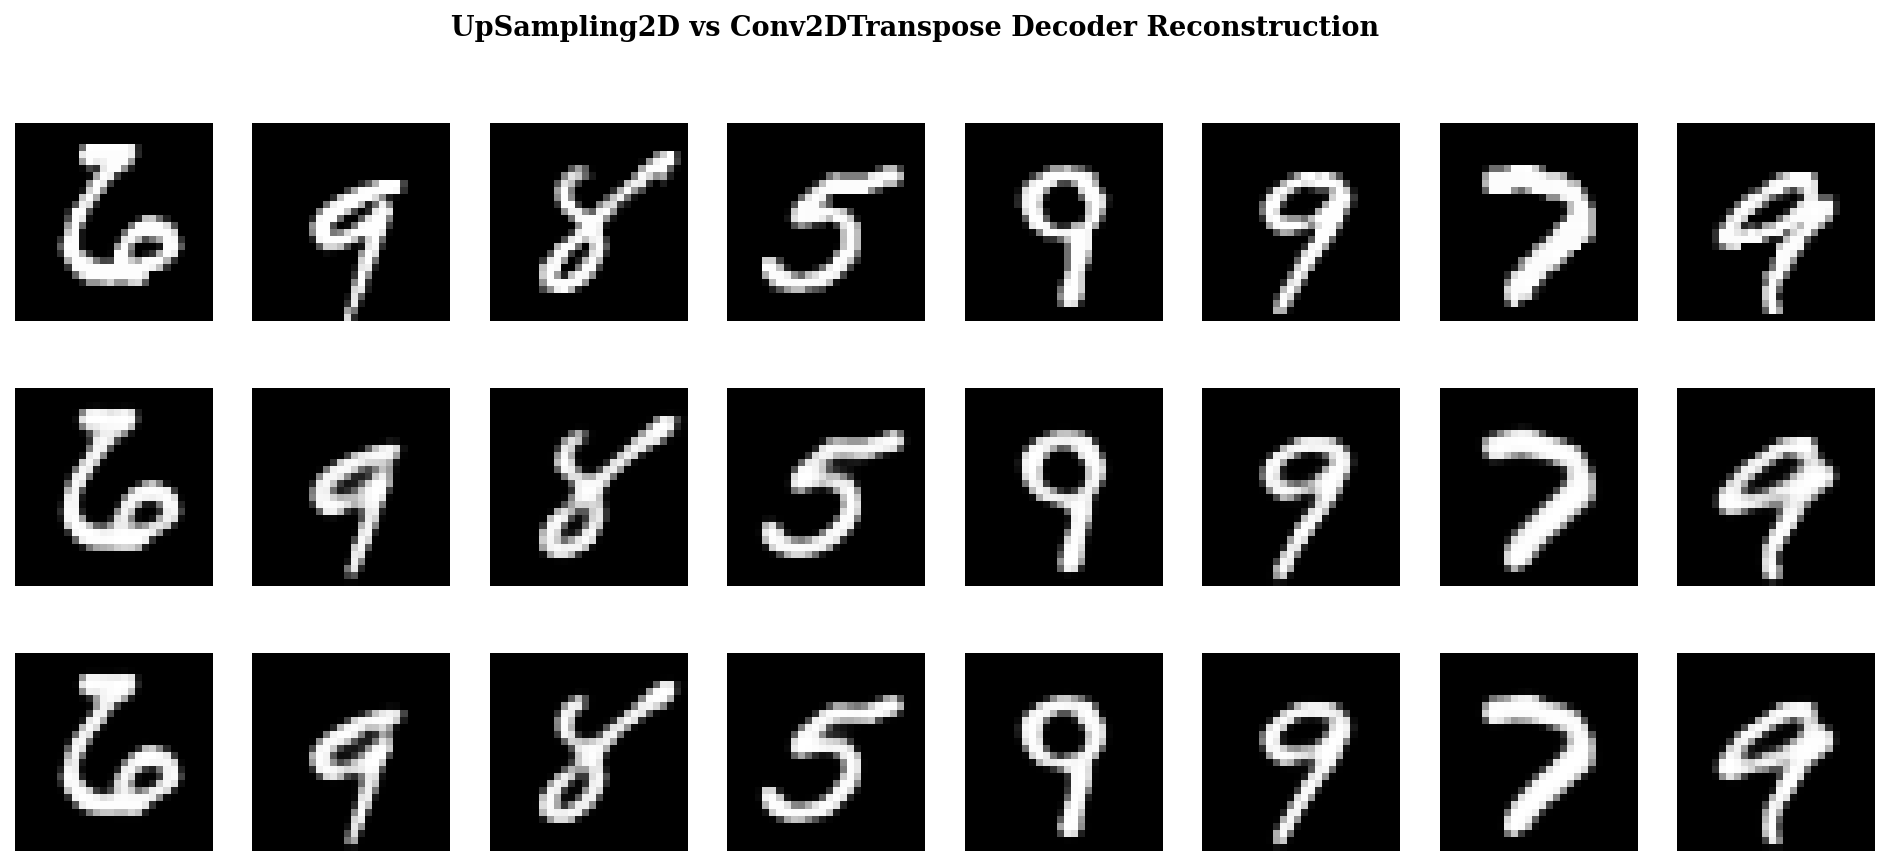
\includegraphics[width=0.9\textwidth]{figures/extra_upsampling_vs_transpose.png}
\caption{Original versus UpSampling2D-decoder reconstruction versus Conv2DTranspose-decoder reconstruction.}
\end{figure}

Conv2DTranspose performs better than UpSampling2D on both metrics with SSIM of 0.980 over 0.975. Conv2DTranspose's upsampling filters are learned and adapted directly to reconstructing, while UpSampling2D repeats pixels first, and then cleans up with convolution later.

\subsection*{27.5 VAE with Latent Dimension 2 vs 8}

Implement a VAE with latent dimension 2 and latent dimension 8 and compare the latent representations.

\begin{center}
\begin{tabular}{|c|c|c|c|}
\hline
Latent Dimension & MSE & MAE & SSIM\\
\hline
2 & 0.044184 & 0.104597 & 0.504711\\
8 & 0.019092 & 0.053513 & 0.795332\\
\hline
\end{tabular}
\end{center}

\begin{figure}[H]
\centering
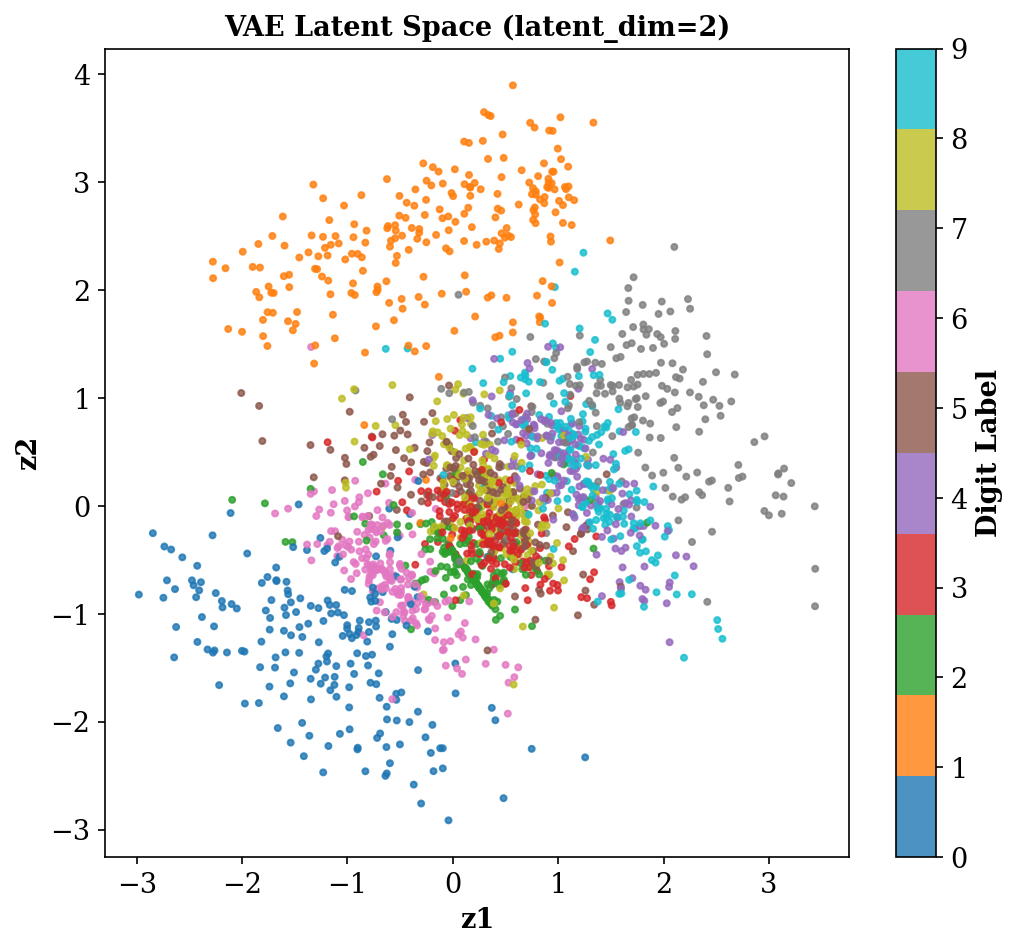
\includegraphics[width=0.6\textwidth]{figures/extra_vae_latent_dim2_space.png}
\caption{2D VAE latent space (latent dimension 2), colored by digit label.}
\end{figure}

Increasing from 2D to 8D reduces MSE greatly, to less than half of its original value, and SSIM increases from 0.505 to 0.795. Encoder separates digit classes clearly, and gets more room to separate them properly. With more dimensions, it gets more room, the encoder separates digit classes more cleanly, but cannot be plotted accurately.

\subsection*{27.6 Effect of Increasing the KL-Loss Contribution ($\beta$-VAE)}

Investigate the effect of increasing the KL-loss contribution using a $\beta$-weighted total loss $\mathcal{L} = \mathcal{L}_{rec} + \beta\,\mathcal{L}_{KL}$.

\begin{center}
\begin{tabular}{|c|c|c|}
\hline
Beta & MSE & SSIM\\
\hline
1.0 & 0.045055 & 0.501015\\
5.0 & 0.047528 & 0.468114\\
10.0 & 0.049827 & 0.418407\\
\hline
\end{tabular}
\end{center}

\begin{figure}[H]
\centering
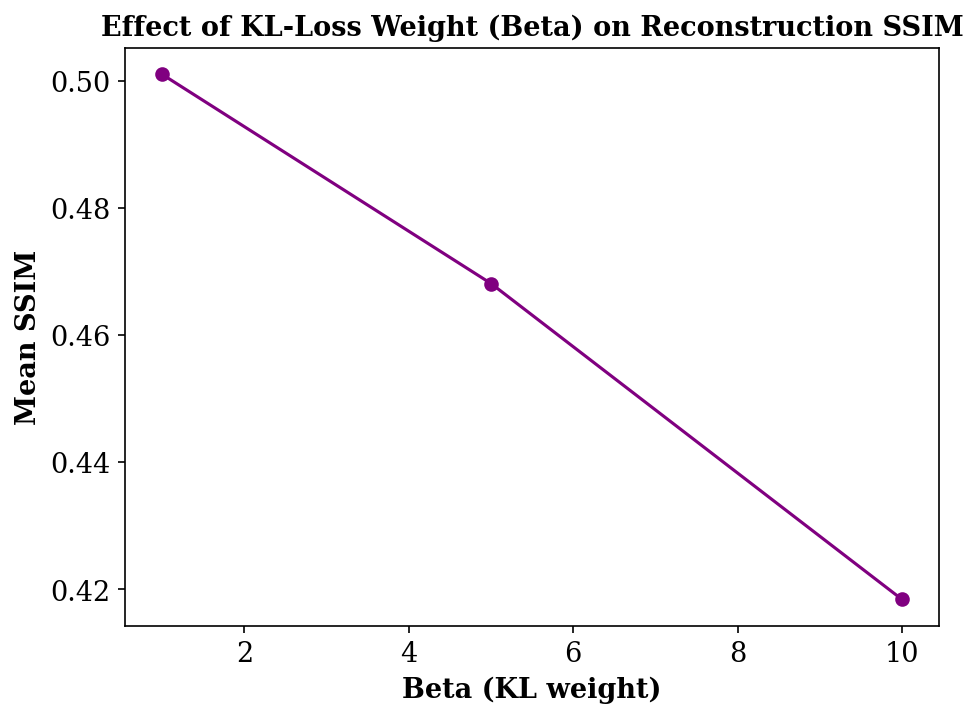
\includegraphics[width=0.6\textwidth]{figures/extra_beta_vae_ssim.png}
\caption{Effect of the KL-loss weight $\beta$ on reconstruction SSIM.}
\end{figure}

SSIM decreases from 0.501 to 0.418, with increase in $\beta$ from 1 to 10, and also increases the MSE. Bigger values of $\beta$ gives heavier weights to the KL term. This pushes the encoder towards plain standard normal prior, and hence leaves lesser room to encode specific details. This shows $\beta$-VAE trade-off, where more regularization for more organized latent space but gives poorer reconstructions.

\subsection*{27.7 Larger Grid of VAE Samples}

Generate a larger grid of 100 VAE samples and discuss diversity.

\begin{figure}[H]
\centering
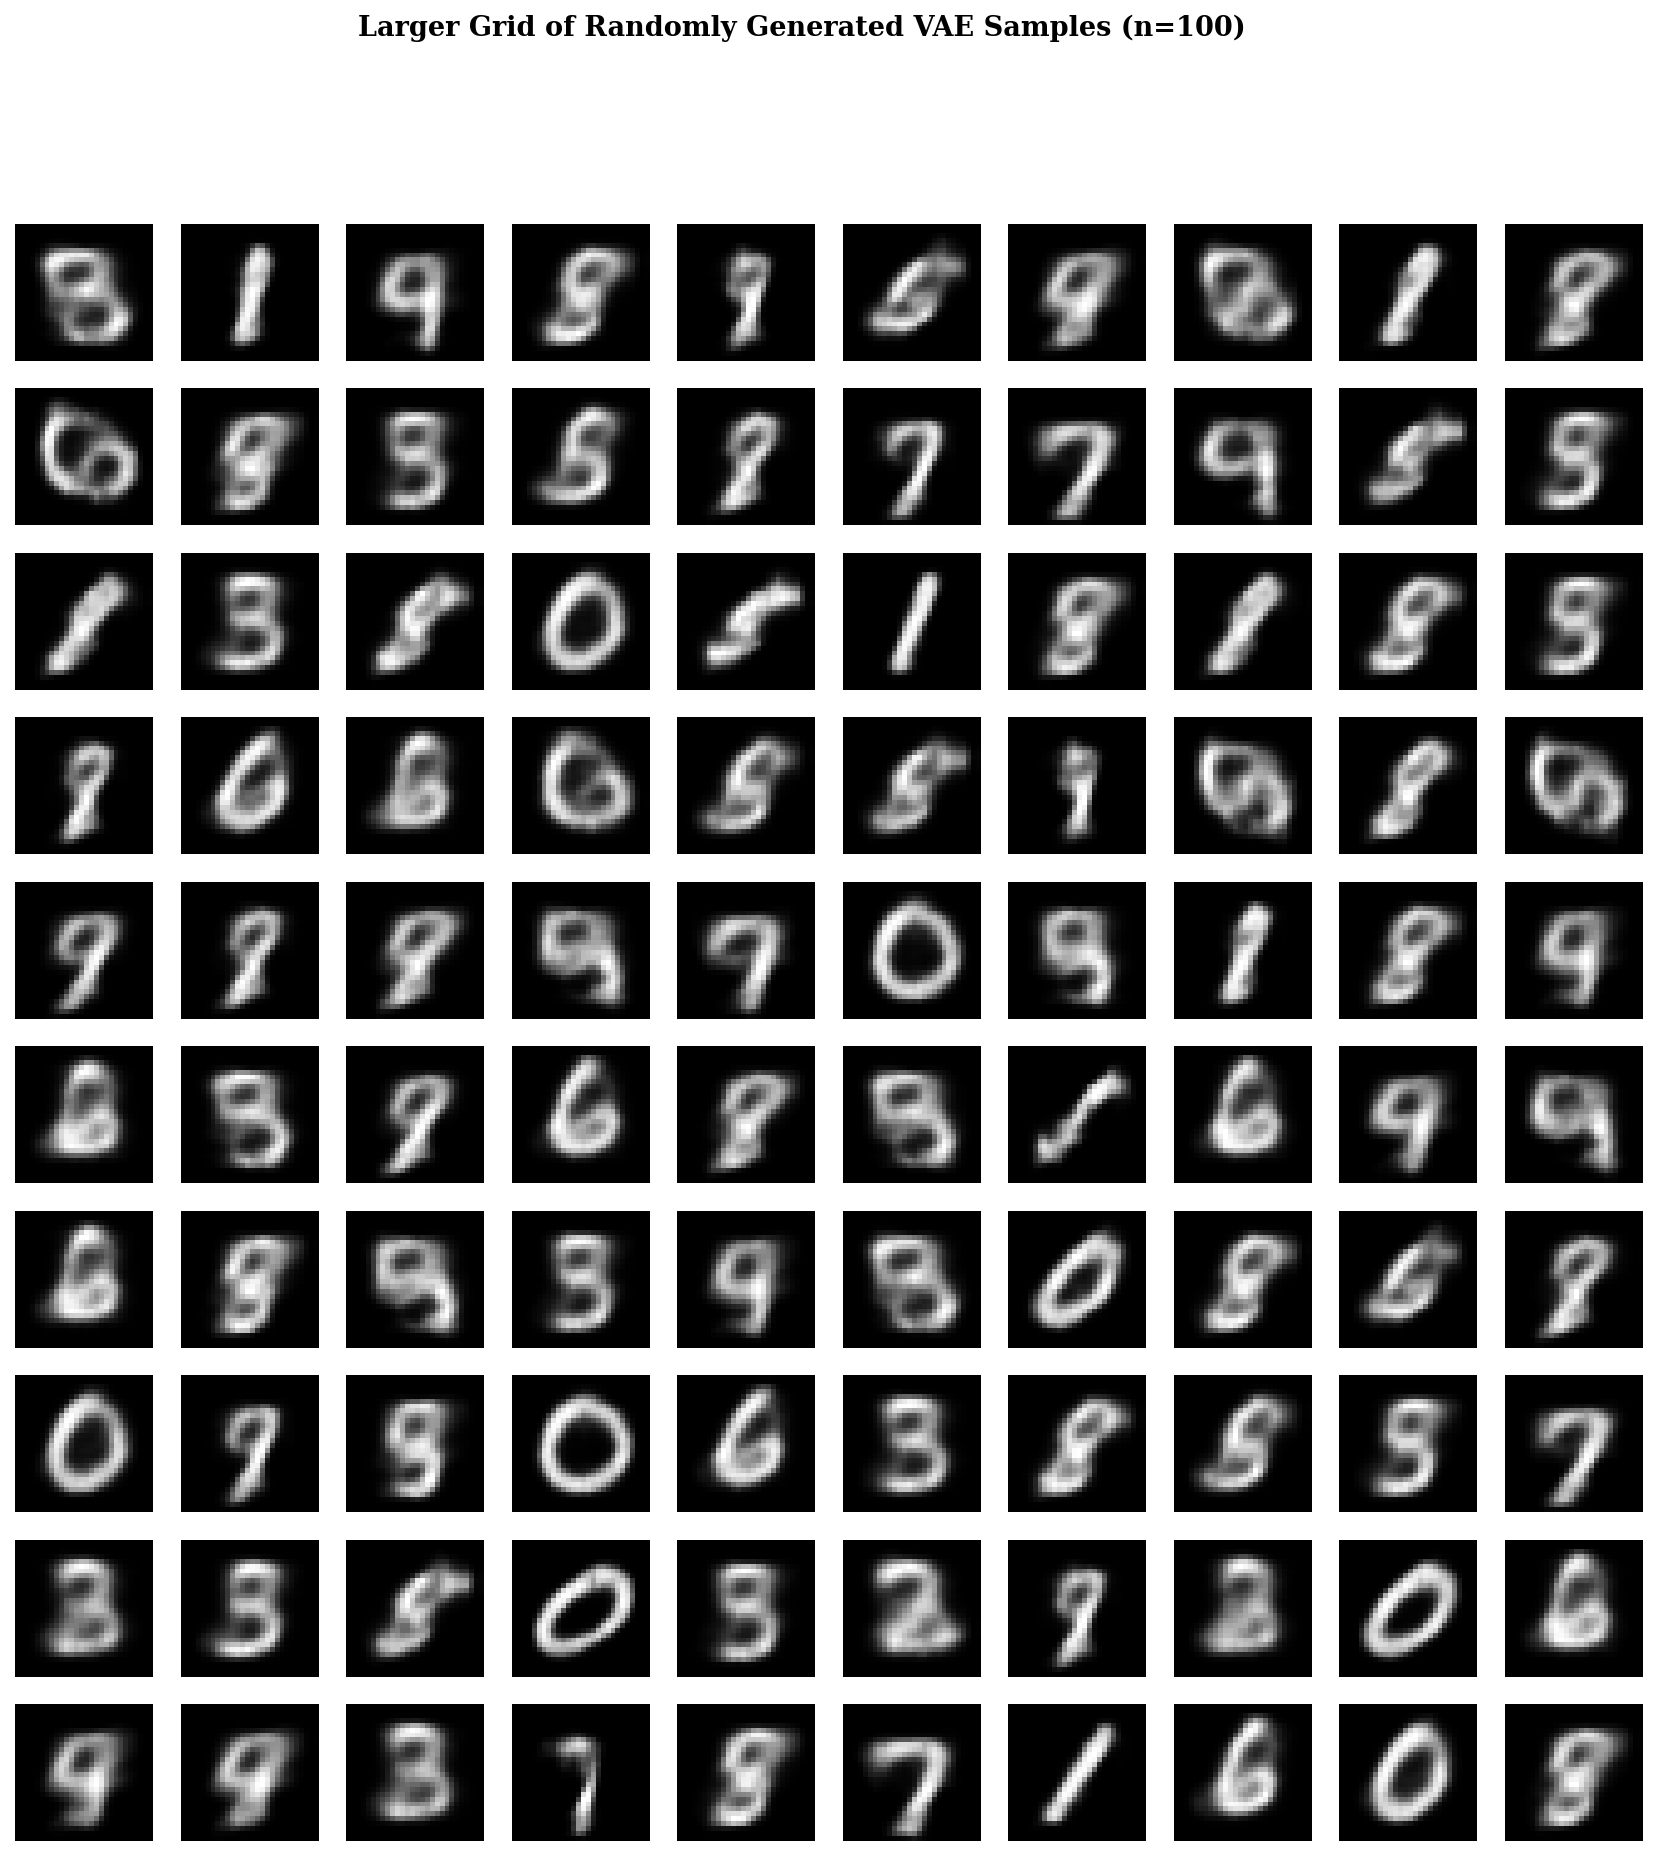
\includegraphics[width=0.6\textwidth]{figures/extra_vae_large_sample_grid.png}
\caption{100 randomly generated VAE samples ($z\sim\mathcal{N}(0,I)$), latent dimension 2.}
\end{figure}

Scaling it to 100 samples still shows multiple different digit shapes and covers a wide range of strokes. It does not repeat the same image multiple times, and shows multiple variations within the same digit. However, the quality of few images look unrecognizable.

\subsection*{27.8 Interpolation Between Two Selected Digit Regions}

Select two digit regions in the latent space (digit 3 and digit 8) and perform interpolation.

\begin{figure}[H]
\centering
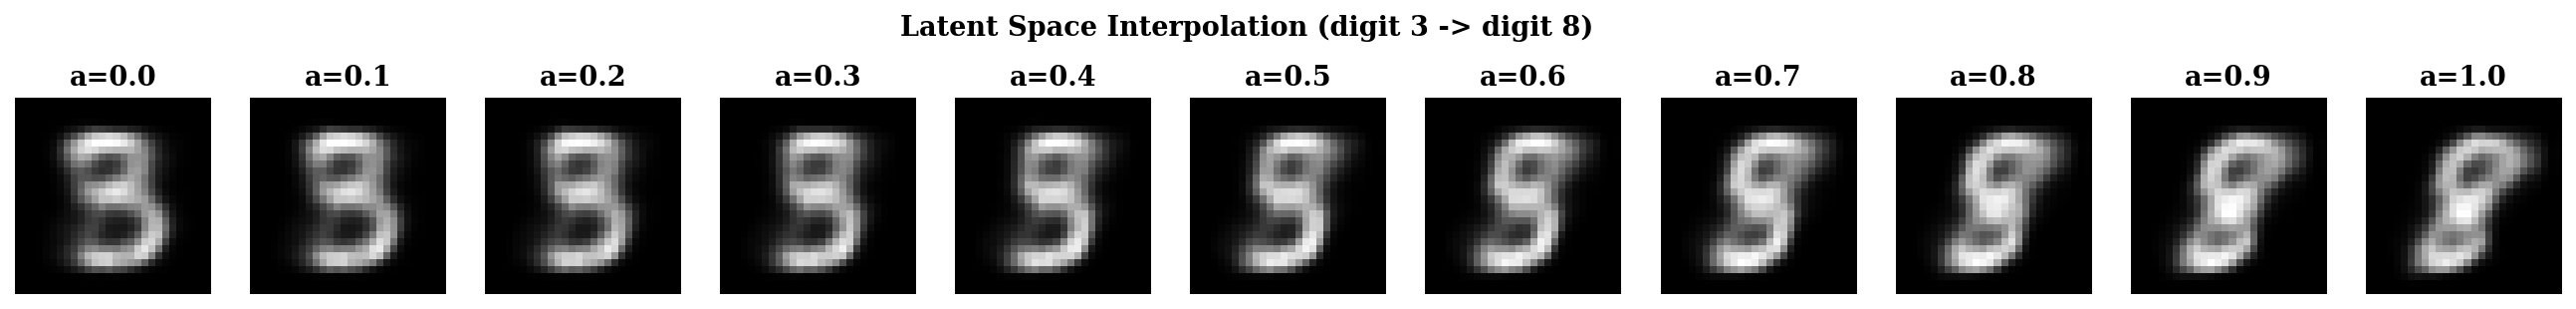
\includegraphics[width=0.95\textwidth]{figures/extra_interpolation_digit3_to_8.png}
\caption{Latent-space interpolation from the encoded latent mean of a digit 3 to that of a digit 8, $\alpha=0$ to $1$ in steps of 0.1.}
\end{figure}

Transition from 3 to 8 happens smoothly, similar to the transition from 0 to 1 before. It happens gradually, and there is no big difference between any two adjacent images, and slowly transitions into 8 from 3.

%%%%%%%%%%%%%%%%%%%%%%%%%%%%%%%%%%%%%%%%%%%%%%%%%%%%%%%%%%%%
\section*{28. Discussion Questions}

\begin{enumerate}

\item \textbf{What is an autoencoder?}\\
An autoencoder is a neural network which reproduces its own input as its output by passing it through a bottleneck. It encodes the data into a smaller version, and then decodes from it to reconstruct the input. Hence the input is the target.\\

\item \textbf{What is the purpose of the encoder?}\\
Encoders compress raw high dimensional inputs into smaller vectors and tries to keep most important features needed for reconstruction. \\

\item \textbf{What is the purpose of the decoder?}\\
Decoders expand the latent vector into an image of higher dimensions, and tries to reconstruct the input image using the important features in the latent space.\\

\item \textbf{What is a latent representation?}\\
Latent representation is an encoded lower dimensional representation of the higher dimensional input image, which contains only the important features and drops very specific or minute details.\\

\item \textbf{Why is the latent representation usually smaller than the input?}\\
Latent representation is the compressed form, which will later be expanded to reconstruct the image. If the image is not compressed and if it is passed directly, then the model simply produces a copy of the image and does not do any reconstruction on its own, and does not learn any important feature, it simply copies.\\

\item \textbf{What happens when the latent dimension is too small?}\\
If the latent dimension is very small,, then the model gets forced to drop a few important features and retains only some important features. Since few important features are missing, the decoding part suffers to reconstruct the input image efficiently, and reconstruction error increases.\\

\item \textbf{What happens when the latent dimension is increased?}\\
If latent dimension is increased, then the model can retain more features and details, and hence the decoding part has more information to reconstruct the input image properly. Hence, reconstruction error decreases and SSIM increases.\\

\item \textbf{Why can a convolutional autoencoder preserve spatial information more effectively?}\\
Convolutional filters retain neighbourhood property, and infer spatial information from pixels. It creates an idea of how a pixel's neighbouring pixels would be. Since the same weights are used throughout the image, the spatial information is retained.\\

\item \textbf{Differentiate an autoencoder and a denoising autoencoder.}\\
Regular autoencoders take a clean image and try to reconstruct it. Denoising autoencoders take in input images with noise, and it tries to remove the noise and retain the core structure of the image.\\

\item \textbf{Why is the clean image used as the target in denoising?}\\
Clean images are used as targets for denoising autoencoders because it helps the model learn to remove the noise and recover true pixels, without reproducing the noise back.\\

\item \textbf{What happens when the noise level is increased?}\\
When noise level is increased, denoising becomes harder, hence MAE and MSE increase, while SSIM decreases. This is because more noise destroys true pixels.\\

\item \textbf{Why are MSE, MAE and SSIM useful for image reconstruction?}\\
MSE and MAE give direct error measures pixel wise. SSIM shows how structurally similar the images are captures how similar the images look.\\

\item \textbf{What is a Variational Autoencoder?}\\
Variational autoencoders are a type of autoencoders which learns the probability distribution over latent space, and tries to generate images with slight variation instead of trying to reconstruct them simply.\\

\item \textbf{How does a VAE differ from a conventional autoencoder?}\\
Variational autoencoders encode each input as a distribution using  $\mu$ and $\log\sigma^2$, and add KL-divergence penalty to the loss. Conventional autoencoders produce one fixed latent vector with no penalty.\\

\item \textbf{Why does a VAE learn a distribution instead of a single latent vector?}\\
VAEs learn distributions which makes the latent space a continuous domain, hence points sampled from the latent space can be decoded into proper images.\\

\item \textbf{What is the reparameterization trick?}\\
Reparameterization trick rewrites the sampling step as $z = \mu + \sigma \odot \epsilon$ with $\epsilon \sim \mathcal{N}(0,I)$. This makes the sampling differentiable everywhere, and hence makes backpropagation possible.\\

\item \textbf{Why is $\epsilon$ sampled from a standard normal distribution?}\\
It supplies randomness required for sampling and also keeping the transformation from $\epsilon$ to $z$ differentiable with respect to the output.\\

\item \textbf{What is the role of KL divergence in the VAE loss?}\\
KL divergence pulls the encoded distributions toward the prior $\mathcal{N}(0,I)$, and keeps the latent space continuous and stops the encoder from collapsing all inputs into a sharp point.\\

\item \textbf{What is the prior distribution used in the VAE?}\\
It is the standard multivariate normal distribution, $p(z) = \mathcal{N}(0, I)$.\\

\item \textbf{Why is a two-dimensional latent space useful for visualization?}\\
2D latent space can be easily plotted into planes, and clustering and structure look easy to distinguish visually.\\

\item \textbf{What does latent-space interpolation demonstrate?}\\
Latent space interpolation shows that latent space is smooth and continuous. It shows that moving between two points is gradual, and there is no huge difference between any two adjacent images.\\

\item \textbf{Why can a VAE generate new images?}\\
VAE regularizes the latent space into a prior distribution. Hence, all points sampled from that distribution is decoded into a new image.\\

\item \textbf{Why might some VAE-generated images be unclear?}\\
If the sampled point is between two digit clusters or in a sparse part of the latent space, the decoder has less information there and produces a blurred input using whatever it has.\\

\item \textbf{What is the difference between reconstruction and generation?}\\
Reconstruction decodes the latent representation of a specific image which exists already. Generation decodes a freshly sampled point from the prior to produce a new image.\\

\item \textbf{Why should test images remain unseen during training?}\\
If test images are seen by the model, then it tries to learn from the test images also, and hence gives better metrics which are not really true. If test images are unseen, then model learns from train images and the testing part gives a genuine metric.\\

\end{enumerate}

%%%%%%%%%%%%%%%%%%%%%%%%%%%%%%%%%%%%%%%%%%%%%%%%%%%%%%%%%%%%
\section*{29. Expected Outcome}

At the end of the experiment, students should be able to demonstrate the
complete image-representation and reconstruction pipeline:

\[
\boxed{
\text{Image}
\rightarrow
\text{Encoder}
\rightarrow
\text{Latent Representation}
\rightarrow
\text{Decoder}
\rightarrow
\text{Reconstructed Image}
}
\]

They should also demonstrate denoising:

\[
\boxed{
\text{Clean Image}
\rightarrow
\text{Noise}
\rightarrow
\text{Denoising Autoencoder}
\rightarrow
\text{Recovered Image}
}
\]

and variational generation:

\[
\boxed{
\text{Image}
\rightarrow
(\mu,\sigma)
\rightarrow
z
\rightarrow
\text{Decoder}
\rightarrow
\text{Generated/Reconstructed Image}
}
\]

The final report should contain both quantitative evaluation and visual
analysis. Numerical performance values must be obtained from the student's
own execution.

%%%%%%%%%%%%%%%%%%%%%%%%%%%%%%%%%%%%%%%%%%%%%%%%%%%%%%%%%%%%
\section*{30. References}

\begin{enumerate}
\item Ian Goodfellow, Yoshua Bengio and Aaron Courville,
\emph{Deep Learning}, MIT Press, 2016.

\item Diederik P. Kingma and Max Welling,
``Auto-Encoding Variational Bayes,'' ICLR, 2014.

\item Pascal Vincent et al.,
``Stacked Denoising Autoencoders: Learning Useful Representations in a Deep
Network with a Local Denoising Criterion,'' Journal of Machine Learning
Research, 2010.

\item Yann LeCun, Corinna Cortes and Christopher J. C. Burges,
``MNIST Handwritten Digit Database.''

\item TensorFlow Documentation:
\url{https://www.tensorflow.org}

\item Keras Documentation:
\url{https://keras.io}

\item scikit-image Documentation:
\url{https://scikit-image.org}
\end{enumerate}

\end{document} 